%% ut-thesis.tex -- document template for graduate theses at UofT
%%
%% Copyright (c) 1998-2013 Francois Pitt <fpitt@cs.utoronto.ca>
%% last updated at 16:20 (EDT) on Wed 25 Sep 2013
%%
%% This work may be distributed and/or modified under the conditions of
%% the LaTeX Project Public License, either version 1.3c of this license
%% or (at your option) any later version.
%% The latest version of this license is in
%%     http://www.latex-project.org/lppl.txt
%% and version 1.3c or later is part of all distributions of LaTeX
%% version 2005/12/01 or later.
%%
%% This work has the LPPL maintenance status "maintained".
%%
%% The Current Maintainer of this work is
%% Francois Pitt <fpitt@cs.utoronto.ca>.
%%
%% This work consists of the files listed in the accompanying README.

%% SUMMARY OF FEATURES:
%%
%% All environments, commands, and options provided by the `ut-thesis'
%% class will be described below, at the point where they should appear
%% in the document.  See the file `ut-thesis.cls' for more details.
%%
%% To explicitly set the pagestyle of any blank page inserted with
%% \cleardoublepage, use one of \clearemptydoublepage,
%% \clearplaindoublepage, \clearthesisdoublepage, or
%% \clearstandarddoublepage (to use the style currently in effect).
%%
%% For single-spaced quotes or quotations, use the `longquote' and
%% `longquotation' environments.


%%%%%%%%%%%%         PREAMBLE         %%%%%%%%%%%%

%%  - Default settings format a final copy (single-sided, normal
%%    margins, one-and-a-half-spaced with single-spaced notes).
%%  - For a rough copy (double-sided, normal margins, double-spaced,
%%    with the word "DRAFT" printed at each corner of every page), use
%%    the `draft' option.
%%  - The default global line spacing can be changed with one of the
%%    options `singlespaced', `onehalfspaced', or `doublespaced'.
%%  - Footnotes and marginal notes are all single-spaced by default, but
%%    can be made to have the same spacing as the rest of the document
%%    by using the option `standardspacednotes'.
%%  - The size of the margins can be changed with one of the options:
%%     . `narrowmargins' (1 1/4" left, 3/4" others),
%%     . `normalmargins' (1 1/4" left, 1" others),
%%     . `widemargins' (1 1/4" all),
%%     . `extrawidemargins' (1 1/2" all).
%%  - The pagestyle of "cleared" pages (empty pages inserted in
%%    two-sided documents to put the next page on the right-hand side)
%%    can be set with one of the options `cleardoublepagestyleempty',
%%    `cleardoublepagestyleplain', or `cleardoublepagestylestandard'.
%%  - Any other standard option for the `report' document class can be
%%    used to override the default or draft settings (such as `10pt',
%%    `11pt', `12pt'), and standard LaTeX packages can be used to
%%    further customize the layout and/or formatting of the document.

%% *** Add any desired options. ***
\documentclass{ut-thesis}

%% *** Add \usepackage declarations here. ***
%% The standard packages `geometry' and `setspace' are already loaded by
%% `ut-thesis' -- see their documentation for details of the features
%% they provide.  In particular, you may use the \geometry command here
%% to adjust the margins if none of the ut-thesis options are suitable
%% (see the `geometry' package for details).  You may also use the
%% \setstretch command to set the line spacing to a value other than
%% single, one-and-a-half, or double spaced (see the `setspace' package
%% for details).
\usepackage{graphicx}
\usepackage{subcaption}
\usepackage{amssymb}
\usepackage{amsmath}
\usepackage{commath}
\usepackage[toc,page]{appendix}

% New commands
\newcommand{\vect}[1]{\boldsymbol{#1}}
%%%%%%%%%%%%%%%%%%%%%%%%%%%%%%%%%%%%%%%%%%%%%%%%%%%%%%%%%%%%%%%%%%%%%%%%
%%                                                                    %%
%%                   ***   I M P O R T A N T   ***                    %%
%%                                                                    %%
%%  Fill in the following fields with the required information:       %%
%%   - \degree{...}       name of the degree obtained                 %%
%%   - \department{...}   name of the graduate department             %%
%%   - \gradyear{...}     year of graduation                          %%
%%   - \author{...}       name of the author                          %%
%%   - \title{...}        title of the thesis                         %%
%%%%%%%%%%%%%%%%%%%%%%%%%%%%%%%%%%%%%%%%%%%%%%%%%%%%%%%%%%%%%%%%%%%%%%%%

%% *** Change this example to appropriate values. ***
\degree{Master of Applied Science}
\department{Civil Engineering}
\gradyear{2019}
\author{Stepan Oskin}
\title{A prototype of a machine learning workflow to classify land use from the housing market dynamics.
Part of a Longitudinal Analysis of housing sales in the Greater Toronto-Hamilton Area.}


%% *** NOTE ***
%% Put here all other formatting commands that belong in the preamble.
%% In particular, you should put all of your \newcommand's,
%% \newenvironment's, \newtheorem's, etc. (in other words, all the
%% global definitions that you will need throughout your thesis) in a
%% separate file and use "\input{filename}" to input it here.


%% *** Adjust the following settings as desired. ***

%% List only down to subsections in the table of contents;
%% 0=chapter, 1=section, 2=subsection, 3=subsubsection, etc.
\setcounter{tocdepth}{2}

%% Make each page fill up the entire page.
\flushbottom


%%%%%%%%%%%%      MAIN  DOCUMENT      %%%%%%%%%%%%

\begin{document}

%% This sets the page style and numbering for preliminary sections.
\begin{preliminary}

%% This generates the title page from the information given above.
\maketitle

%% There should be NOTHING between the title page and abstract.
%% However, if your document is two-sided and you want the abstract
%% _not_ to appear on the back of the title page, then uncomment the
%% following line.
%\cleardoublepage

%% This generates the abstract page, with the line spacing adjusted
%% according to SGS guidelines.
\begin{abstract}
%% *** Put your Abstract here. ***
%% (At most 150 words for M.Sc. or 350 words for Ph.D.)
    There is ample evidence of the role of land use and transportation interactions in determining urban spatial structure.
    The new data sources introduced by increased digitization of human activity, such as Teranet's dataset of real estate sales, offer opportunities for development of integrated urban models or studies conducting longitudinal analysis of changes in land value distributions.
    To facilitate this, data from various sources (Census, TTS, etc.) needs to be merged at the land parcel level to enhance datasets with additional attributes, while maintaining the ease of data storage and retrieval.
    In addition to that, accurate land use information needs to be added to Teranet records to allow separating sales data by major property types.
    This master's thesis proposes a prototype of a workflow to augment Teranet's dataset with data from multiple sources and use machine learning to classify land use of each Teranet record based on the housing market dynamics.
\end{abstract}

%% Anything placed between the abstract and table of contents will
%% appear on a separate page since the abstract ends with \newpage and
%% the table of contents starts with \clearpage.  Use \cleardoublepage
%% for anything that you want to appear on a right-hand page.

%% This generates a "dedication" section, if needed -- just a paragraph
%% formatted flush right (uncomment to have it appear in the document).
%\begin{dedication}
%% *** Put your Dedication here. ***
%\end{dedication}

%% The `dedication' and `acknowledgements' sections do not create new
%% pages so if you want the two sections to appear on separate pages,
%% uncomment the following line.
%\newpage  % separate pages for dedication and acknowledgements

%% Alternatively, if you leave both on the same page, it is probably a
%% good idea to add a bit of extra vertical space in between the two --
%% for example, as follows (adjust as desired).
%\vspace{.5in}  % vertical space between dedication and acknowledgements

%% This generates an "acknowledgements" section, if needed
%% (uncomment to have it appear in the document).
%\begin{acknowledgements}
%% *** Put your Acknowledgements here. ***
%\end{acknowledgements}

%% This generates the Table of Contents (on a separate page).
\tableofcontents

%% This generates the List of Tables (on a separate page), if needed
%% (uncomment to have it appear in the document).
%\listoftables

%% This generates the List of Figures (on a separate page), if needed
%% (uncomment to have it appear in the document).
%\listoffigures

%% You can add commands here to generate any other material that belongs
%% in the head matter (for example, List of Plates, Index of Symbols, or
%% List of Appendices).

%% End of the preliminary sections: reset page style and numbering.
\end{preliminary}


%%%%%%%%%%%%%%%%%%%%%%%%%%%%%%%%%%%%%%%%%%%%%%%%%%%%%%%%%%%%%%%%%%%%%%%%
%%  Put your Chapters here; the easiest way to do this is to keep     %%
%%  each chapter in a separate file and `\include' all the files.     %%
%%  Each chapter file should start with "\chapter{ChapterName}".      %%
%%  Note that using `\include' instead of `\input' will make each     %%
%%  chapter start on a new page, and allow you to format only parts   %%
%%  of your thesis at a time by using `\includeonly'.                 %%
%%%%%%%%%%%%%%%%%%%%%%%%%%%%%%%%%%%%%%%%%%%%%%%%%%%%%%%%%%%%%%%%%%%%%%%%

%% *** Include chapter files here. ***
\chapter[Introduction]{Introduction} \label{ch:introduction}

\section{Introduction} \label{sec:intro}
\chapter[Background information]{Background information} \label{ch:background}

\section{Chapter 2: transportation and land use, land registration in Canada and Teranet} \label{sec:chapter_2_intro}

This chapter discusses the complex interaction of land use and transportation, provides a brief overview of the history of development of land use-transportation (LUT) models, presents some legal and historical background for Teranet's dataset of real estate transactions and finishes with discussing challenges of working with Teranet's data and the proposed solution.

\section{Land Use and Transport (LUT) models} \label{sec:evolution_of_models_of_urban_systems}

\subsection{Complexity of urban systems and "wicked" problems} \label{subsec:complexity_and_wicked_problems}

In her famous 1961 book, Jane Jacobs\cite{Jacobs1961} described a city as "a problem in organized complexity";
since then, many other researchers have remarked that urban systems exhibit complex behaviour\cite{Batty2008, Bettencourt2013}.
Complexity of a system can be defined as a state or quality of being intricate or complicated.
For a system to be complex is not necessarily the same as to be complicated;
complex systems can be simple, i.e.\ governed by a single equation.
Complexity of a system has to do with the intrinsic ability of a system to surprise us with its behaviour;
that the system is hard to understand, despite the mechanics of it being relatively simple.

In 1973, a little over a decade after Jacobs, Rittel and Webber\cite{Rittel1973} presented a path-breaking conceptualization;
this conceptualization characterized urban planning problems as "wicked" problems: problems which cannot be definitively described and for which it makes no sense to talk of "optimal solutions".
In their paper, Rittel and Webber stated that such "wicked" problems are never "solved", and that the focus instead becomes on iteratively "re-solving" the problems over and over.
More than 40 years after their original publication, Rittel and Webber's ideas remain relevant to the policy sciences today: there is an intense interest in the nature of "wicked" problems and the complex tasks of identifying their scope, viable responses, and appropriate mechanisms and pathways to improvement\cite{Crowley2017}.
Interaction between land use and transportation, which is discussed in the following section, presents a prime example of urban complexities and "wicked" problems.

\subsection{Transportation-land use cycle} \label{subsec:transportation_land_use_cycle}

Among the reasons why transportation and land use interaction is "wicked" are such aspects as pluralism of expectations among stakeholders, institutional complexity in policy making, and scientific uncertainty\cite{Noto2015}.
More importantly, there is a fundamental link between transportation and urban form: urban form has an enormous impact on the type and cost of transportation systems needed to serve residents of a metropolitan area\cite{Kelly1994}.
Transportation, in turn, influences land development and location choices of people and firms, and thus completes the formation of a feedback relationship that Stover and Koepke\cite{Stover1988} referred to as a cycle.
Interconnections between points (activities) in space can be perceived through the medium of the transportation system\cite{Miller1998}

Figure~\ref{fig:idealized_integrated_urban_model} illustrates the complex interactions between land use and transportation system as summarized by Miller, Kriger and Hunt\cite{Miller1998}.

\begin{figure}[hbt!]
    \centering
    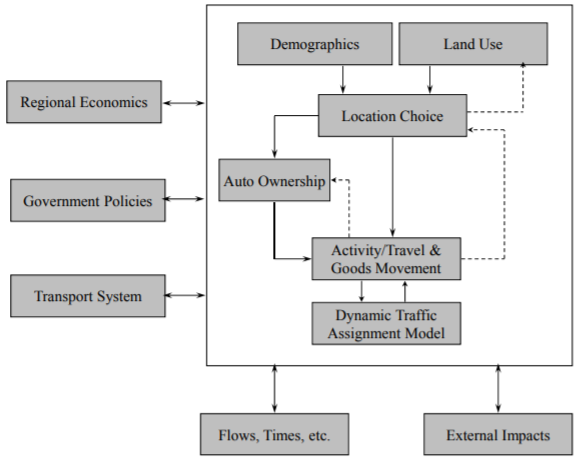
\includegraphics[width=0.7\linewidth,trim=0 0 0 0,clip]{miller_idealized_urban_model.png}
    \caption{An Idealized Integrated Urban Model System, adapted from Miller, Kriger and Hunt\cite{Miller1998}.}
    \label{fig:idealized_integrated_urban_model}
\end{figure}

Many different types of models are used in planning, such as demand forecasting models projecting traffic or ridership, or land use models projecting and distributing population and jobs within an area.
At an earlier stage of model development, some analysts argued that there is no significant link between transportation and land use, given the near-ubiquity of the transportation (road) network\cite{Miller1998}.
However, the unprecedented urban growth of the 21st century introduced new challenges for urban systems such as extreme road congestion, equity of access to jobs and services among low-income households, energy scarcity, environmental and GHG impacts from transportation systems and public health impacts of land use patterns\cite{Miller2018b,Moeckel2017}.

It became apparent that these "transport problems" cannot be solved through transportation policies and investment alone, that the physical design of the city at the "macro" and "micro" scale critically interfaces with the demand for and performance of the transportation system.
In addition, to accurately assess the costs and benefits of an expensive long-term transportation infrastructure investment, "feedback" effects of these investments on urban form, land values, property taxes, quality of life, etc.
need to be quantified and included in evaluation and decision making.
Thus, today there is a steadily growing recognition within the urban policy field that the interaction between transportation and land use does exist and does matter\cite{Miller2018b}.

%TODO change the end of 1st sentence
In the context of models, integrated urban models (IUMs) aim to capture the complex relationship between urban systems such as transportation and land use more accurately.
Integrated land use-transportation models combine travel demand forecasting and land use forecasting functions and recognize that the distribution of population and jobs depends, in part, on transportation accessibility.
The reverse is also true, and thus integrated models incorporate feedback relationship between transportation and land use, with economic decisions by households and firms acting as one of the links between the two systems\cite{Miller1998}.

\subsection{Evolution of LUT models} \label{subsec:evolution_of_lut_models}

The history of treating cities as systems via simulation models of transportation and land use dates back to 1950s when General System Theory and Cybernetics came to be applied in the softer social sciences\cite{Batty2008}.
The first operational simulation model that truly integrated land use and transportation is considered to be A Model of Metropolis built in 1964 by Ira S. Lowry for the Pittsburgh region based on economic base theory\cite{Lowry1964}.
It was a highly aggregate model based on theories of spatial interaction, such as the gravity model that was popular in quantitative geography and transportation planning at the time\cite{Bouchard1965}.
Models based on spatial interaction framework continued to be developed through mid-1980s, until developments in random utility theory allowed researchers to describe choices among discrete alternatives, such as the choice of travel mode, and generate models based on the study of disaggregate behaviour\cite{Iacono2008}.

Figure~\ref{fig:lut_model_evolution} provides the general overview of chronological development of LUT models summarized by Iacono\cite{Iacono2008}.

\begin{figure}[hbt!]
    \centering
    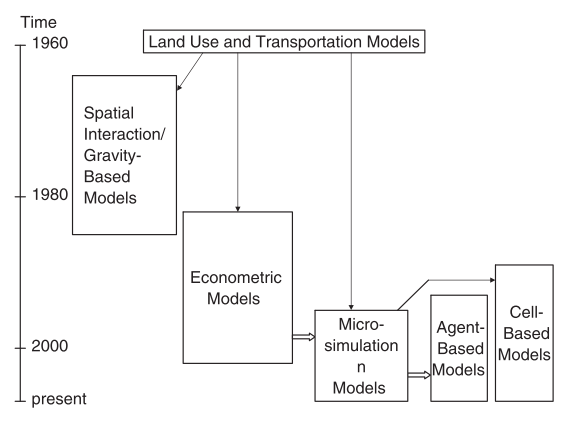
\includegraphics[width=0.7\linewidth,trim=0 0 0 0,clip]{lut_models_evolution.png}
    \caption{Chronological development of LUT models summarized by Iacono\cite{Iacono2008}.}
    \label{fig:lut_model_evolution}
\end{figure}

The modeling paradigm has changed fundamentally in the early 1990s along with the advances in computing power and efficiency of data storage.
Urban systems used to be viewed as hierarchical and centrally organized equilibrium structures, or "top-down".
Instead, now they were considered to be structured from the "bottom-up", dynamically retaining their integrity through interactions of numerous microelements\cite{Batty2008}.
A new broad class of LUT models that could fall under the title of "microsimulation" began to be developed.
It included such classes of models as activity-based travel, cell-based models, and multi-agent models, and more recently comprehensive urban microsimulation models that fully reflect the dynamics of changes in the population and the urban environment\cite{Iacono2008}.
%TODO check last sentence

"Micro" in the microsimulation implies that the model must be highly disaggregated spatially, socio-economically and in its representation of processes.
"Simulation" implies that the model must be numerical, stochastic, have an explicit time dimension, and "evolve" into the end state rather than "solve for it"\cite{Miller2018c}.
An example of such model has been developed by the University of Toronto ILUTE team;
their product is an integrated urban model capable of microsimulating urban demographic evolution, housing markets and travel behaviour over extended periods of time\cite{Miller2018a}.
The ILUTE system and some of the ways for its future improvement are discussed in the following section.

\subsection{ILUTE and HoMES model systems} \label{subsec:ilute}

The Integrated Land Use, Transportation, Environment (ILUTE) model system is an agent-based microsimulation model for greater Toronto-Hamilton area;
it includes such components as land use, activity/travel, urban economics, auto ownership, demographics and emissions/energy use.
It uses disaggregate models of spatial socioeconomic processes to evolve the state of the greater Toronto\textendash Hamilton area from a known base case to a predicted end state in 1-year time steps.
The system state is defined in terms of the individual persons, households, dwelling units, firms, etc.
that collectively define the urban region being modeled\cite{Miller2011}.

ILUTE model simulates the evolution of an urban region's spatial form, demographics, travel behavior and economic structure over time.
Many markets are of interest within ILUTE, such as housing, labour, commercial, real estate, etc.) and are modeled via microsimulation.
The model aims to capture the dynamics of these markets through disaggregated representations.
For example, in the housing market component of ILUTE, houses are auctioned off one dwelling at a time to interested bidders in a disaggregate implementation of Martinez' Bid Choice theory\cite{Martinez1992}.

The Housing Market Evolutionary System (HoMES) is the updated housing market module for the ILUTE model system.
HoMES is a disaggregate, agent-based microsimulation of the owner-occupied housing market that evolves the residential location of households over time and includes the endogenous supply of housing by type and location, as well as the endogenous determination of sales prices and rents.

An overview of the framework of housing market supply, demand and clearing mechanisms utilized in HoMES provided by Rosenfield et al.\cite{Rosenfield2013} is presented on figure~\ref{fig:homes_framework}

\begin{figure}[hbt!]
    \centering
    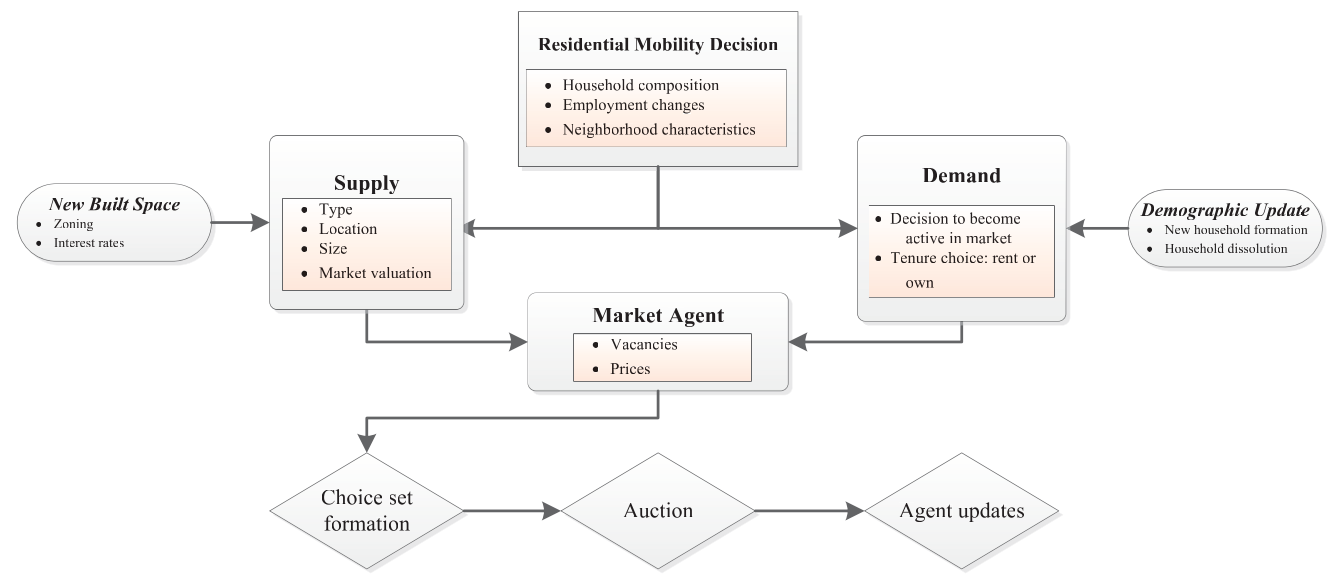
\includegraphics[width=0.99\linewidth,trim=0 0 0 0,clip]{homes_framework.png}
    \caption{Framework of housing market supply, demand and clearing mechanisms used in HoMES module of ILUTE, as summarized by Rosenfield et al.\cite{Rosenfield2013}.}
    \label{fig:homes_framework}
\end{figure}

Among the major barriers to implementation of integrated urban models since their introduction were such aspects as data hungriness and computational requirements\cite{Miller1998}.
However, continuing methodological advances, such as cost-effective High Performance Computing (HPC), detailed GIS-based datasets and machine learning methods, mean that former barriers now represent opportunities for model system development.
In the case of ILUTE and HoMES, one of the possibilities for further improvement is the use of new data sources to update the housing market model.
One of these new data sources, Teranet's dataset of land registry records, and main challenges of working with it are discussed in section~\ref{sec:new_data_sources_and_their_challgenges}.

\section{New data sources and their challenges} \label{sec:new_data_sources_and_their_challgenges}

\subsection{Further improvement of integrated urban models} \label{subsec:further_improvement_of_iums}


As an increasing amount of aspects of human life becomes digitalized, a wealth of new data is produced and can be used to model and analyze dynamics of urban systems\cite{Arribas-Bel2014, Chen2016}.
An example of such digitalization of human activity is the introduction of the Province of Ontario Land Registration Information System (POLARIS) in 1985 by the Government of Ontario\cite{TeranetEnterprisesInc.} that will be discussed in the following section.
Introduction of POLARIS lead to the creation of an extensive dataset of real estate transactions (land registration records) by the Teranet Enterprises Inc.
This dataset offers a very fine resolution of housing market dynamics across both time and space, which can be beneficial for updating and testing microsimulation models, but it also presents challenges to work with that will be discussed in section~\ref{subsec:teranet_ontario} of this chapter;
the chapter concludes with the proposed solution to address one of the main challenges of working with Teranet's data.

\subsection{POLARIS: electronic system of land registration in Ontario} \label{subsec:land_reg_system_canada}

All land owned in Canada is registered in a public land registry in the applicable province.
Each province and territory in Canada has its own land registry system, whether it is a land titles system, a registry system or a combination of both, with each system having its own rules.
The registry system is a public record of documents evidencing transactions affecting land.
In the land titles system, the applicable provincial government determines the quality of the title, and essentially guarantees (within certain statutory limits) the title to, and interests in, the property.
As of 2015, most common law provinces and territories in Canada were using the land titles system or were in the process of converting from a registry system to a land titles system\cite{McKean2015}.

As of 2015, the Province of Ontario has largely converted from registry systems to a land titles system.
In 1985, the Government of Ontario initiated the Province of Ontario Land Registration Information System (POLARIS) pilot project for the purposes of the conversion between systems and records automation.
The Land Registration Reform Act (Ontario)\cite{TheGovernmentofOntario1990} was introduced in 1990 to facilitate electronic search and registration of properties and the automation of paper-based records.
POLARIS was built by the Province to house and process electronic land records, which in turn lead to the creation of an extensive dataset of land registration records managed by Teranet Enterprises Inc.
Today, POLARIS is the search/registration and property maintenance system for all automated land records in Ontario.

\subsection{The Teranet-Ontario Partnership, Teranet's data and its challenges} \label{subsec:teranet_ontario}

In 1991, the Government of Ontario established a partnership with Teranet, a Toronto-based organization, founded the same year, which provides e-services to legal, real estate, government, financial, and healthcare markets.
The partnership was established to convert Ontario's land registration system to a more modernized electronic title system.
The project involved taking a 200-year-old paper-based system and creating a database with electronic records for more than five million parcels of land.
Teranet converted all qualified Registry properties in Ontario to the Land Titles system and automated existing paper Land Titles parcels.
As a result, 99.9\% of property in Ontario was parcelized and administered under the Land Titles system.
Teranet fully automated the conversion of millions of paper-based documents and records into the Ontario Electronic Land Registration System (ELRS)\cite{TeranetEnterprisesInc.2019}.


Teranet dataset presents an extensive historical record of real estate transactions recorded in the Province of Ontario since the beginning of XIX century.
However, when it comes to using new data sources in social studies, along with opportunities there are also challenges present.
For example, these data sources can have issues with the quality of the data, might require a specific set of skills to take advantage of these data sources, or might not be suitable for traditional methods meant for traditional data\cite{Arribas-Bel2014}, all of which are true in the case of Teranet's dataset.

One of the major attributes missing from the available version of Teranet's dataset is the information about the type of property being transacted, with records of various residential, commercial and industrial properties all being mixed together in the same dataset.
At the same time, Teranet records have timestamps (dates) and location information (x and y coordinates) and thus can be joined to variety of other urban data sources, such as Census demographics, Transportation Tomorrow Survey (TTS) and parcel-level land use information.
It is possible to derive this attribute from additional related sources of information, such as detailed land use or Census demographics.
However, joining these data sources together requires additional considerations, as they use different spatial units and are available at different temporal spans, as will be discussed in chapter~\ref{ch:spatial_and_temporal_relationships_between_urban_data}.


\section{Chapter summary} \label{sec:background_summary}

The fundamental link between transportation and urban form creates a feedback relationship between land development, travel needs, viability of alternative modes, accessibility, and other important characteristics of the urban transportation system.
Numerous "top-down" and "bottom-up" models have been designed to analyze and forecast the behaviour of urban regions and interaction of their transportation and land use systems.
Since urban systems are complex in nature and require "re-solving" over and over, data science process models present a good fit for this task with their iterative structure.

Increased digitization of human activity, such as introduction of POLARIS land registration system by the Government of Ontario in 1985, produce a wealth of new information that can be used to study interaction between land use and transportation at a fine spatial and temporal scale.
Teranet's dataset of real estate transactions presents a wealth of information on the housing market of Ontario and can be used for empirical studies of transportation-land use interaction.
However, along with the opportunities, the new data sources also present new challenges.
Teranet's dataset has some data quality issues that need to be addressed and might require special skills to work with due to its size.
But most importantly, it is very limited in the number of features available for each transaction.

One of the major attributes missing from the available version of Teranet's dataset is the information about the type of property being transacted, with records of various residential, commercial and industrial properties all being mixed together in the same dataset.
At the same time, Teranet records have timestamps (dates) and location information (x and y coordinates) and thus can be joined to variety of other urban data sources, such as Census demographics, Transportation Tomorrow Survey (TTS) and parcel-level land use information.
It is possible to derive this attribute from additional related sources of information, such as detailed land use or Census demographics.
However, joining these data sources together requires additional considerations, as they use different spatial units and are available at different temporal spans, as will be discussed in chapter~\ref{ch:spatial_and_temporal_relationships_between_urban_data}.

\chapter{Spatial and temporal relationships between data sources} \label{ch:spatial_and_temporal_relationships}

The second phase of CRISP-DM process model for data mining projects is data understanding;
this chapter discusses the nature of spatial and temporal relationships of different data sources that are used in this master's thesis.
As was discussed in section~\ref{sec:teranet_challenges_solution}, one of the main challenges of working with Teranet's data is the lack of available features.
At the same time, Teranet records have timestamps (dates) and location information (x and y coordinates) and thus can be joined to a variety of other urban data sources, such as Census demographics, Transportation Tomorrow Survey (TTS) and parcel-level land use information.
However, as will be discussed in this chapter, these data sources use different spatial units and are available at different temporal spans;
therefore, special consideration must be taken when joining data from these sources with respect to their temporal and spatial relationships to ensure semantic interoperability.

Different data sources joined to Teranet's dataset are described in this chapter, the implementation of the spatial and temporal relationships via the standardized data preparation workflow in Python and a PostgreSQL relational database are described in chapter~\ref{ch:data_preparation}.

\section{Description of data sources used} \label{sec:description_of_data_sources}

The following data sources were combined into the GTHA housing market database that was created as a part of this master's thesis:

\begin{enumerate}
    \item Teranet's dataset

    Due to the introduction of POLARIS by the Province of Ontario in 1985 (discussed in section~\ref{sec:polaris}), Teranet's dataset includes a complete population of real estate transactions recorded in Ontario from 1985 up to October of 2017 (records prior to 1985 appear to be incomplete, see figure~\ref{fig:teranet_time_series}).
    Since Teranet's dataset has a high number of records, it can be used to investigate aspects relating to the housing market at a very fine spatial and temporal scale.


    \begin{figure}[hbt!]
        \centering
        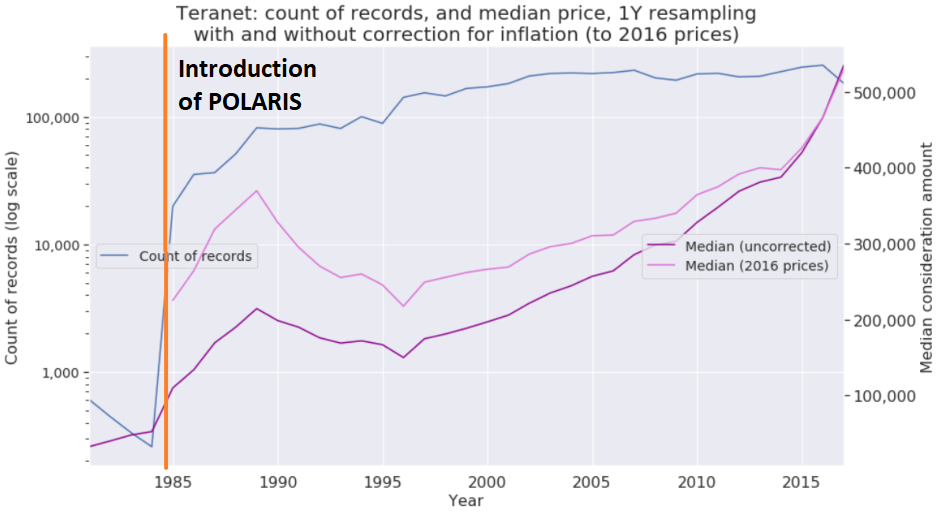
\includegraphics[width=1\linewidth,trim=0 0 0 0,clip]{teranet_time_series.png}
        \caption{Time series of total count of Teranet records within GTHA boundary (log scale, left y-axis) and their median consideration amount (right y-axis), resampled by 1-year intervals.
        It can be seen that there is a dramatic increase in the total count of records between 1984 and 1985, which coincides with the introduction of POLARIS electronic land registration system by the Government of Ontarion in 1985, which was discussed in section~\ref{sec:polaris}.
        Teranet records prior to 1985 appear to be incomplete.}
        \label{fig:teranet_time_series}
    \end{figure}

    \item Select variables from the Census of Canada

    One of the major sources of demographic and statistical data in Canada are the datasets collected under the national Census program.
    Census datasets provide valuable insights into the latest economic, social and demographic conditions and trends in Canada and are used to plan important public services.
    Statistics Canada collects every five years the national Census of Canada and disseminates the information by a range of geographic units, also referred to as "Census geography"\cite{MapandDataLibrary2019}.

    \item Select variables from the Transportation Tomorrow Survey (TTS)

    Another major source of information for most transportation planning studies concerned with Southern Ontario is the Transportation Tomorrow Survey (TTS), an origin-destination travel survey\cite{DataManagementGroup2014}.
    The Transportation Tomorrow Survey (TTS), undertaken every five years since 1986, is a cooperative effort by local and provincial government agencies to collect information about urban travel in southern Ontario.
    TTS represents a retrospective survey of travel taken by every member (age 11 or over) of the household during the day previous to the telephone or web contact.
    The information collected and the method of collection has remained relatively consistent over the seven surveys;
    TTS survey data includes characteristics of the household, characteristics of each person in the household, and details of the trips taken by each member of the household, including details on any trips taken by transit\cite{Ashby2018}.

    \item Land use from DMTI Spatial Inc.\ by year (2001-2014)

    DMTI Spatial Inc., a Digital Map Products company, is a major provider of location based information in Canada.
    DMTI has been providing industry leading enterprise Location Intelligence solutions for more than a decade to Global 2000 companies and government agencies\cite{DMTISpatialInc.2014}.

    \item Detailed land use information from University of Toronto's Department of Geography collected in 2012 and 2013

    The detailed land-use data provided by University of Toronto's Department of Geography is a combination of parcel boundaries (from Teranet) and manually coded land-use data produced using Google maps and streetviews;
    it was collected by Prof.\ Andre Sorensen and Prof.\ Paul Hess's research project.

\end{enumerate}

\section{Spatial relationships between data sources} \label{sec:spatial_relationships}

Most urban areas are divided into zones or planning areas on the basis of maintaining similar population sizes and following built or natural boundaries like roads or rivers.
Census geography follows a certain hierarchy defined by Statistics Canada, with the largest top-level divisions being provinces and territories, and the lowest-tier divisions to which Census data is disseminated being Dissemination Areas (DAs)\cite{StatisticsCanada2018}.
Statistics Canada defines a Dissemination Area as a small area composed of one or more neighbouring dissemination blocks, roughly uniform in population size targeted from 400 to 700 persons to avoid data suppression\cite{StatisticsCanada2015}.

To simulate the changes in accessibility, metropolitan regions are usually broken down into a set of small geographic zones, similar (or in many cases identical) to the set of zones used for regional travel forecasting.
For TTS variables, the finest level of spatial aggregation is that of the Traffic Zone, also referred to as the Traffic Analysis Zone (TAZ).
A Traffic Zone is a polygon which typically falls along the centre line of roads or the natural geographic boundaries\cite{DataManagementGroup2019}.
Not as a rule, but TAZ zones roughly follow Census tract boundaries, which are slightly bigger than DA boundaries.
Figure~\ref{fig:da_taz_difference} presents an example of TAZ polygons overlaid with Census DA boundaries.

\begin{figure}[hbt!]
    \centering
    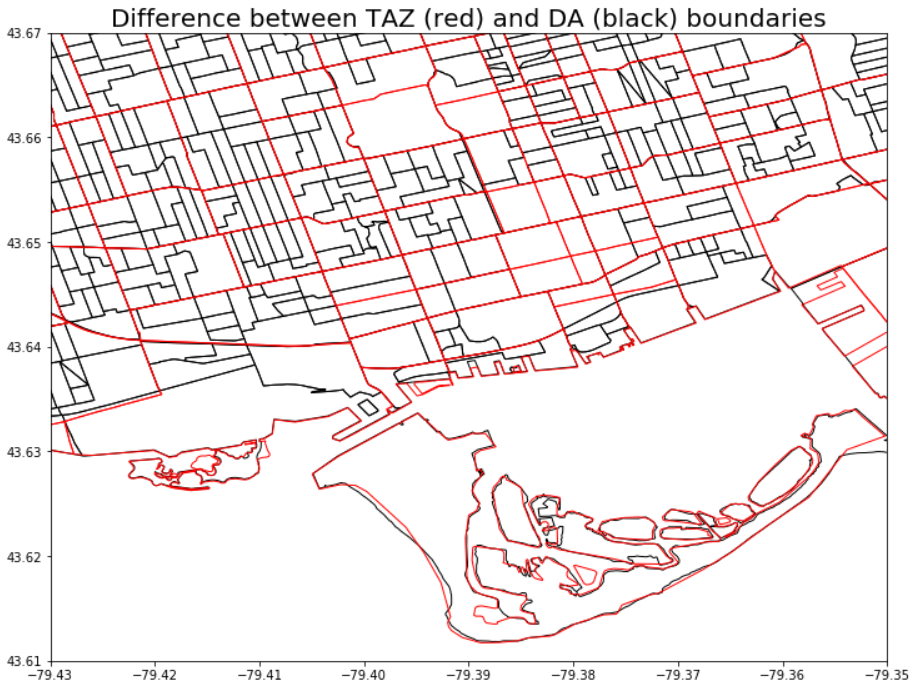
\includegraphics[width=0.7\linewidth,trim=0 0 0 0,clip]{da_taz_difference.png}
    \caption{Spatial relationship between datasets: difference between Traffic Analysis Zones (TAZ, red) and Census Dissemination Area (DA, black).}
    \label{fig:da_taz_difference}
\end{figure}

TTS data has been collected for changing TAZ boundaries, or in other words, different zone systems due to growing population and expanding extents of the survey in the GTHA region over the years.
To make the TTS data consistent for comparing over all years from 1986 to 2016, the Data Management Group (DMG) at the University of Toronto Transportation Research Institute (UTTRI), the custodian of the dataset derived from TTS, made all surveys available in the 2001 zone system, for convenience of researchers (any zone system could have been chosen for that matter).
UTTRI used the 2001 TAZ system to model travel times for the GTHA on EMME for all TTS years based on the origin-destination trip data collected in the survey.
The travel time data was used to create further transportation accessibility variables.

Land use data collected by DMTI and by the Department of Geography uses the spatial unit of a parcel polygon.
Teranet records have attributes representing x and y coordinates matching parcel centroids.

\vspace{5mm}

Below is the summary of spatial units used by the data sources that were combined into the GTHA housing market database, designed and implemented as a part of this master's thesis:

\begin{itemize}
    \item Point data
    \begin{itemize}
        \item Teranet
    \end{itemize}
    \item Parcel-level data (polygons)
    \begin{itemize}
        \item detailed land use from the Department of Geography
        \item land use from DMTI
    \end{itemize}
    \item DA-level data (polygons)
    \begin{itemize}
        \item Census variables
    \end{itemize}
    \item TAZ-level data
    \begin{itemize}
        \item TTS variables
    \end{itemize}
\end{itemize}

When joining these data sources, difference in spatial units needs to be respected, which can be more challenging when spatially joining polygons with polygons, since it might require area-weighted spatial interpolation of data to a common unit of analysis.
In addition, polygon-based data can also vary with time, as is the case with DMTI's land use information, which is available by year.
To simplify relating different polygon-based data sources with each other, all of them can be brought together to a single level of time-indexed points, such as Teranet transactions.
This allows flexibility in combining data from polygon-based data sources to a common point level while maintaining the integrity of spatial and temporal relationships through polygon-to-point spatial joins.
Implementation of these relationships is described in chapter~\ref{ch:data_preparation}, temporal relationships between different data sources are described in the following section.

\section{Temporal relationships between data sources} \label{sec:termporal_relationships_between_datasets}

In addition to using different spatial units, data sources joined with Teranet's dataset are available at different temporal spans:
\begin{itemize}
    \item Teranet records have individual timestamps (date) on each record
    \item Census and TTS variables are sampled once in 5 years
    \item DMTI's land use data is available by year and covers a time span from 2001 to 2014
    \item Detailed land use from the Department of Geography was collected at a single point in time during the summers of 2012 and 2013
\end{itemize}

Temporal matching between Teranet records and DMTI data can be done directly: DMTI land use for each year from 2001 to 2014 can be spatially joined with a subset of Teranet records from the corresponding year;
such approach would ignore changes of land use types that occur within a year, but would recognize land use changes between the years for which DMTI land use data is available.
Since the detailed land use provided by the Department of Geography was collected at a single point in time, it can be joined to all Teranet records;
however, it should be kept in mind that this land use data will be the most accurate around its time of collection in 2012 and 2013, and will become increasingly less accurate with an increase of the temporal span of Teranet records.

\begin{figure}[hbt!]
    \centering
    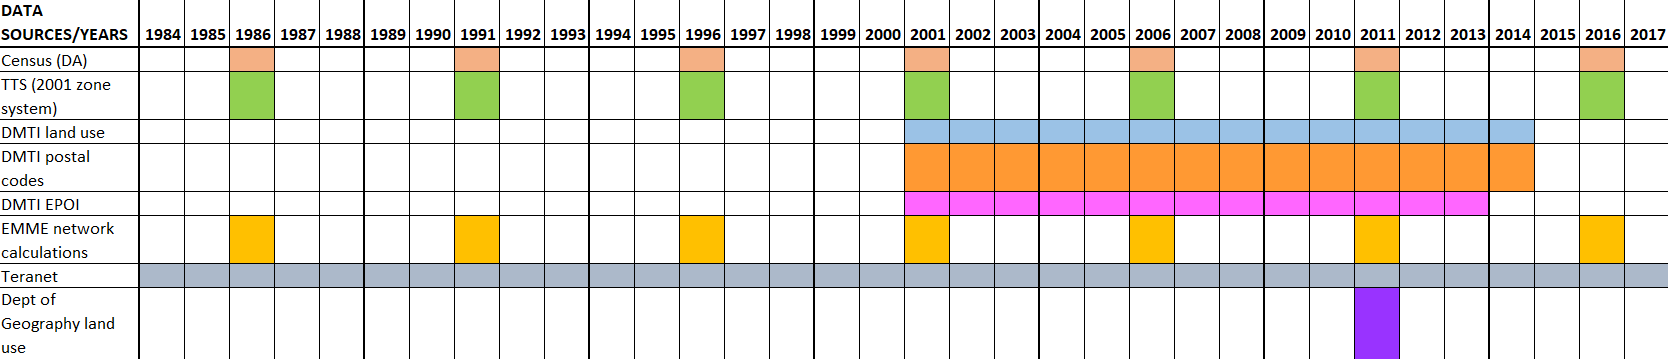
\includegraphics[width=1\linewidth,trim=0 0 0 0,clip]{temporal_spans.png}
    \caption{Temporal spans of data sources used in the GTHA housing market database.}
    \label{fig:temporal_spans}
\end{figure}

\vspace{5mm}

As for Teranet and Census / TTS variables, they can be matched in a number of ways:

\begin{enumerate}
    \item Direct match with appropriate Teranet subsets
    \begin{itemize}
        \item match Census / TTS variables only with Teranet records from the corresponding year (for example, Teranet records from 2016 matched with 2016 Census / TTS variables)
        \item benefits:
        \begin{itemize}
            \item Census / TTS variables would be composed of the actual values recorded by the survey
        \end{itemize}
        \item disadvantages:
        \begin{itemize}
            \item limited use of Teranet data since only records from Census / TTS years can be matched
        \end{itemize}
    \end{itemize}
    \item Interpolation of discrete Census / TTS variables
    \begin{itemize}
        \item discrete Census / TTS variables can be turned into continuous via interpolation
        \item benefits:
        \begin{itemize}
            \item closest temporal match between Teranet and Census / TTS variables
        \end{itemize}
        \item disadvantages:
        \begin{itemize}
            \item additional assumptions need to be made for each Census / TTS variable
        \end{itemize}
    \end{itemize}
    \item Assign temporal spans to each Census / TTS survey as new features to Teranet records
    \begin{itemize}
        \item each Census / TTS survey is assigned a temporal span of 5 years;
        this 5-year span represents a group of Teranet records to which variables from this survey can be matched (for example, Census variables of 2016 are matched with Teranet record from 2014 to 2018)
        \item benefits:
        \begin{itemize}
            \item avoid interpolation assumptions
        \end{itemize}
        \item disadvantages:
        \begin{itemize}
            \item step-change in Census / TTS variables
        \end{itemize}
    \end{itemize}
\end{enumerate}

To avoid additional interpolation assumptions and use the actual values recorded from Census and TTS surveys, the third option has been chosen for matching Teranet records with Census / TTS variables.
Each Census / TTS survey is assigned a 5-year time span centered at the survey year (i.e., 2014--2018 for 2016 survey year) and new foreign keys are introduced to Teranet records to allow matching with 5-year time spans of Census / TTS variables.
Implementation of temporal relationships for Teranet records will be described in chapter~\ref{ch:data_preparation}.
Figure~\ref{fig:temporal_spans} presents the temporal spans assigned to each data source for joining with Teranet records.

\section{Chapter summary} \label{sec:data_sources_summary}

Variables that can be joined to augment Teranet's dataset, such as Census and TTS surveys and parcel-level land use data, are defined using different spatial units and are available at varying temporal spans.
These relationships need to be respected when combining variables from these data sources into a single dataset to ensure semantic interoperability.
The integrity of spatial relationships can be ensured by spatially joining all polygon-based data sources to Teranet points.
Temporal relationships between DMTI land use and Teranet sales records are incorporated by performing separate spatial join operations for each annual DMTI land use dataset with a corresponding Teranet subset.
For Census and TTS variables, additional foreign keys are introduced assigning 5-year spans to each Teranet record corresponding to a Census / TTS survey;
these foreign keys indicate which Teranet records should be joined to a particular Census or TTS survey.
Implementation of these relationships via a standardized data preparation workflow in Python and a PostgreSQL relational database are described in chapter~\ref{ch:data_preparation}.

\chapter{Data preparation} \label{ch:data_preparation}

The "wicked" nature of transportation and land use interaction introduced in chapter~\ref{ch:background} dictates the need to iteratively "re-solve" transportation and land use planning problems instead of focusing on finding some single "optimal solution".
This approach resembles the methodologies typically employed for data science projects, where the sequence of steps is iterated over, producing a more meaningful solution on each new iteration of the cycle, as defined by such process models as CRISP-DM\cite{Shearer2000}.
Similarly, data preparation can be followed in a linear manner, but is very likely to be iterative in nature\cite{Brownlee2013}.

\vspace{5mm}

Data preparation plays a critical role in research projects:

\begin{itemize}
    \item it can determine the success of applications of machine learning algorithms
    \item it is a prerequisite for any meaningful analysis
    \item it is often required to allow the introduction of constraints necessary for implementation of RDBMS
\end{itemize}

\vspace{5mm}

To facilitate easy modification and replication of the data preparation process for data sources related to the GTHA housing market, a streamlined data preparation workflow using Python via a series of jupyter notebooks has been established as a part of this master's thesis.
It accomplishes three main objectives:
\begin{itemize}
    \item clean Teranet dataset and correct its records for consistency
    \item introduce new keys that allow efficient joining of other data sources such as Census or TTS, while maintaining the integrity of spatial and temporal relationships that were discussed in chapter~\ref{ch:spatial_and_temporal_relationships}
    \item engineer new features that can be used by the machine learning algorithm along with the features from the joined datasets to classify land use, which will be discussed in chapter~\ref{ch:ml_workflow}
\end{itemize}

This chapter introduces the concepts of ''Tidy Data'' and database normalization and outlines the standardized data preparation workflow for all data sources related to the GTHA housing market.

\section{Tidy data and database normalization} \label{sec:db_norm_tidy_data}

Hadley Wickham in his paper ''Tidy Data''\cite{Wickham2014} formalized the way how a shape of the data can be described and what goal should be pursued when formatting data.
The tidy data standard is closely related to Edgar F. Codd's relational algebra and has been designed to facilitate initial exploration and analysis of the data, and to simplify the development of data analysis tools that work well together.
As an integral part of his relational model, Codd\cite{Codd1990} proposed a process of database normalization, or restructuring of a relational database in accordance with a series of so-called normal forms in order to reduce data redundancy and improve data integrity.
Normalization entails organizing the columns (attributes) and tables (relations) of a database to ensure that their dependencies are properly enforced by database integrity constraints.
The principles of ''tidy data'' essentially reformulate Codd's ideas in statistical language.

According to Wickham\cite{Wickham2014}, ''tidy data'' is a standard way of mapping the meaning of a dataset to its structure.
A dataset is ''messy'' or ''tidy'' depending on how rows, columns and tables are matched up with observations, variables and types.

\vspace{5mm}

In ''tidy data'':
\begin{enumerate}
    \item Each variable forms a column.
    \item Each observation forms a row.
    \item Each type of observational unit forms a table.
\end{enumerate}

This is Codd's 3rd normal form\cite{Codd1990}, but with the constraints framed in statistical language, and the focus put on a single dataset rather than the many connected datasets common in relational databases.
''Messy data'' is any other arrangement of the data.

\vspace{5mm}

The structure of Teranet's dataset conforms with the ''Tidy data'' format.
Contrary to Teranet, tables with combined selected Census and TTS variables have variables for different Census and TTS years recorded as columns.
This needs to be addressed by ''melting'' these tables and introducing a new attribute 'year' to be used as a part of a composite foreign key when joining with Teranet records.

\vspace{5mm}

Census and TTS tables were ''melted'' into the ''tidy data'' format:
\begin{itemize}
    \item each Census / TTS variable now forms a single column
    \item each value of a variable is indexed by a composite primary key constituting of spatial identifier and year of the survey
    \item spatial identifiers are 'DAUID' or 'TAZ\_O' (unique identifier for Dissemination Areas or Traffic Analysis Zones introduced in section~\ref{sec:spatial_relationships})
\end{itemize}

Introduction of new foreign keys is described in the following section.

\section{Introduction of new keys and attributes via spatial and temporal relationships} \label{sec:introduction_of_new_keys}

As no combination of columns constitutes a candidate key for Teranet records (unique identifier to be used in RDBMS), a surrogate key (artificial unique identifier for RDBMS) is added to the Teranet dataset via a new attribute 'transaction\_id'.
Thus, Teranet's dataset fits into a normalized database, with the new attribute 'transaction\_id' as its primary key.
As was discussed in section~\ref{sec:db_norm_tidy_data}, the ''melted'' Census and TTS tables have composite primary keys consisting of a unique spatial identifier ('DAUID' or 'TAZ\_O', respectively) and the year of the survey.

To implement the spatial and temporal relationships between the data sources discussed in chapter~\ref{ch:spatial_and_temporal_relationships}, a number of new foreign keys needed to be introduced to Teranet records.
The new foreign keys either represent spatial identifiers (such as 'dauid' or 'taz\_o', corresponding to DA or TAZ within which a Teranet record is located), or an attribute identifying the year of the Census or TTS survey to which this Teranet record can be joined.
Foreign keys representing spatial identifiers are added through a series of spatial joins while foreign keys identifying temporal spans are produced based on temporal relationships established in section~\ref{sec:termporal_relationships_between_datasets}.

\vspace{5mm}

New spatial identifiers were introduced to each Teranet record via a series of spatial joins:
\begin{enumerate}
    \item 9'039'241 Teranet points were joined with 9'182 polygons of Dissemination Areas (DAs) for GTHA used by Census variables
    \begin{itemize}
        \item Teranet records with coordinates falling outside of GTHA boundary were filtered out
        \item From the original 9'039'241 records, 6'803'691 remained in the dataset
        \item New foreign keys 'dauid', 'csduid' and attribute 'csdname' were added to each Teranet record
    \end{itemize}
    \item 6,803,691 Teranet points were joined with 1,716 polygons of Traffic Analysis Zones (TAZ) used by TTS variables
    \begin{itemize}
        \item New foreign key 'taz\_o' was added to each Teranet record
    \end{itemize}
    \item 6,803,691 Teranet points were joined with 525 polygons of Forward Sortation Areas (FSA) and 555,668 polygons of postal geography from DMTI's Platinum Postal Geography Suite
    \begin{itemize}
        \item New foreign keys 'fsa' and 'pca\_id' and attribute 'postal\_code\_dmti' were added to each Teranet record
        \item These keys are not currently used for joining any variables, but were added to expand the potential for relating datasets
    \end{itemize}
    \item 6,803,691 Teranet points were joined with 1,664,862 polygons of parcel-level detailed land use provided by the Department of Geography
    \begin{itemize}
        \item New foreign keys 'pin\_lu', 'landuse' and 'prop\_code' were added to each Teranet record
        \item Foreign keys 'landuse' and 'prop\_code' are codes that can be converted to land use categories that were used by the Department of Geography for GTA and Hamilton, respectively
        \item For records from Hamilton, 'prop\_code' was converted to categories used by GTA land use and reassigned to 'landuse', bringing GTA and Hamilton records to a single system of land use categories
    \end{itemize}
    \item Subsets of Teranet points were joined with corresponding yearly polygons of parcel-level land use from DMTI
    \begin{itemize}
        \item New attribute 'dmti\_lu' was added to each Teranet record
    \end{itemize}
\end{enumerate}

\begin{figure}[hbt!]
    \centering
    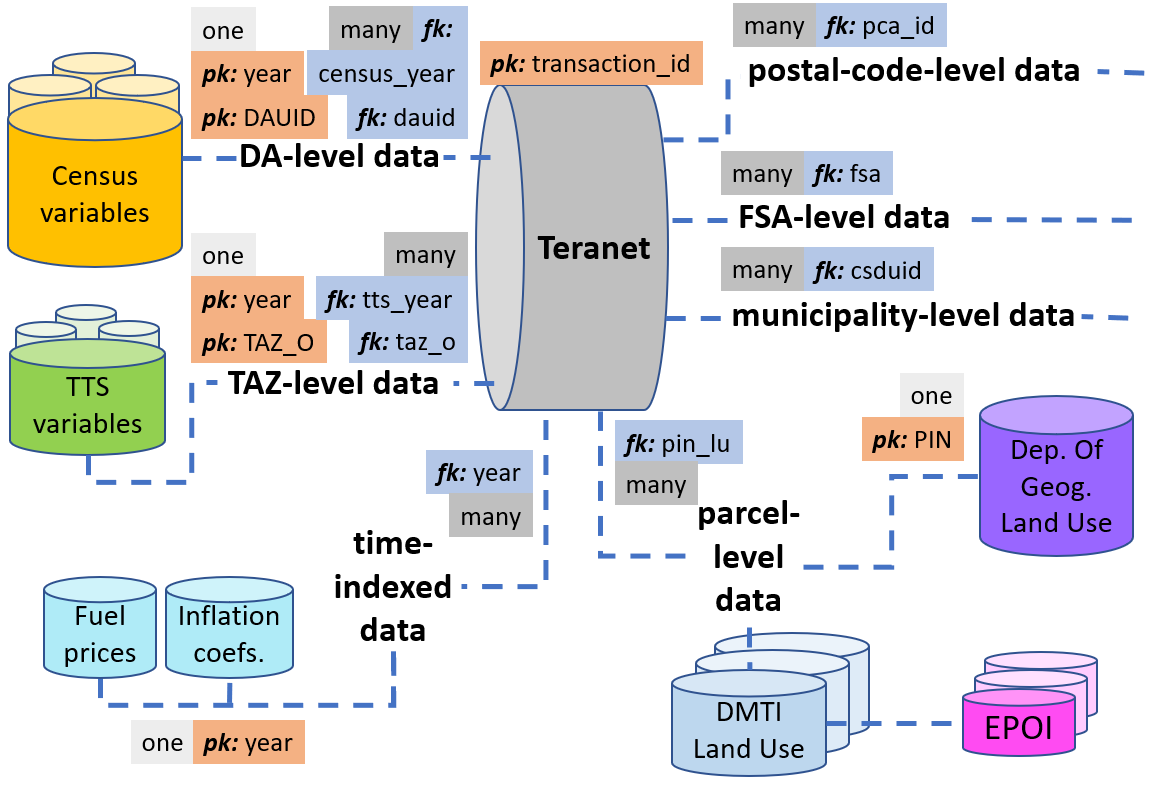
\includegraphics[width=1\linewidth,trim=0 0 0 0,clip]{data_relations.png}
    \caption{Relationships between datasets introduced during data preparation were then used to set up referential integrity constraints of the new PostgreSQL database for GTHA housing market data.}
    \label{fig:data_relations}
\end{figure}

Foreign keys representing temporal identifiers are generated from the registration date of each Teranet record, matching each year of Teranet records to a corresponding 5-year span covered by a Census or TTS survey, as was discussed in section~\ref{sec:termporal_relationships_between_datasets}.
Diagram of relationships between datasets and their primary and foreign keys is presented on figure~\ref{fig:data_relations}

Following the steps described above ensures that the integrity of spatial and temporal relationships is maintained when combining attributes from different data sources at Teranet transaction level.
For example, Teranet records from 2007 would be spatially joined with DMTI land use data from 2007, and are matched by their attributes 'census\_year' and 'tts\_year' to Census and TTS variables from 2006 Census and TTS surveys.
Census and TTS variables can be joined by appropriate 'dauid' and 'taz\_o' (composite foreign keys are used when joining), and thus all data sources can be spatially and temporally aligned at the level of Teranet transactions.

Relationships introduced via the operations described in this section formulate referential integrity constraints that have been used to set up a PostgreSQL database of GTHA housing market data.

\section{Dealing with outliers} \label{sec:outliers}

Outliers in both the high and the low end of the price distribution are present in Teranet's dataset:
\begin{itemize}
    \item there is a high number of transactions with very low consideration amounts (starting from a few dollars) that most likely represent transactions recording gifts of property, where some symbolic consideration amount has been used
    \item at the same time, since the dataset includes all types of property transactions, some records have very high values (in the range of hundreds of millions and billions of dollars) that most likely correspond to transactions recording sales of large commercial and industrial properties or whole residential buildings
\end{itemize}

The large spike can be seen on the low end of the distribution of consideration amount presented on figure~\ref{fig:bottom_outliers}; this spike corresponds to gift transactions with symbolic prices.

\begin{figure}[ht]
    \centering
    \begin{subfigure}{\linewidth}
        \centering
        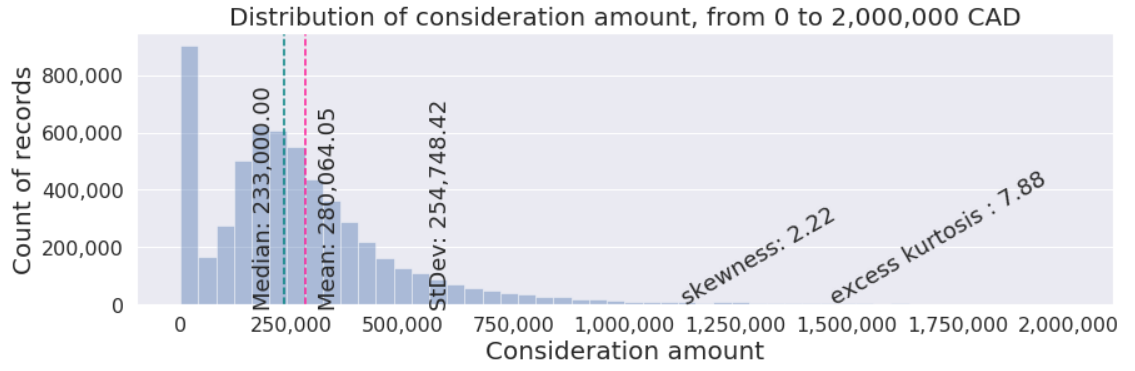
\includegraphics[width=.8\linewidth]{price_dist_raw.png}
        \caption{From 0 to 2'000'000 CAD}
    \end{subfigure}

    \begin{subfigure}{\linewidth}
        \centering
        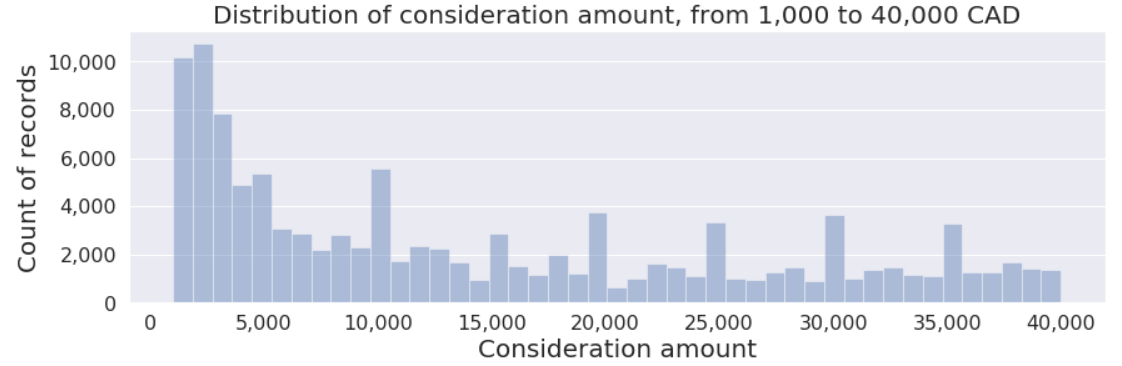
\includegraphics[width=.8\linewidth]{price_dist_zoom.png}
        \caption{From 0 to 40'000 CAD}
    \end{subfigure}
    \caption{Outliers at the bottom end of the price distribution most likely represent gift transactions.
    Large spike can be seen on the low end of the distribution.
    Since no clear break can be identified, 10'000 CAD was used as the cut-off threshold to filter Teranet records.}
    \label{fig:bottom_outliers}
\end{figure}

Since low outliers represent transactions that are not useful for analysis, they were removed from the dataset.
However, there is no way to establish what constitutes a reasonable bottom cut-off threshold, as there is no criteria available and there is no distinct break in the price distribution.
Since there seems to be en exceptionally large spike of transactions with consideration amount under 10'000 CAD, they were considered to be low outliers and were removed from Teranet's dataset, further reducing the number of records from 6,803,691 to 5,188,513.

In the case of outliers on the high end of the price distribution, they most likely correspond to transactions of expensive commercial and industrial property or whole residential buildings.
Since these transactions are useful for research questions concerning commercial and industrial property, they are left in the dataset and instead are marked with special features.
Since, again, there is no clear criteria for what would constitute an outlier, instead of using a single criterion, 7 different attributes are added that describe whether a record belongs to outliers according to a particular condition.
Examples of boxplots produced from two different criteria used to mark top outliers are presented on figure~\ref{fig:top_outliers}.

\begin{figure}[ht]
    \centering
    \begin{subfigure}{\linewidth}
        \centering
        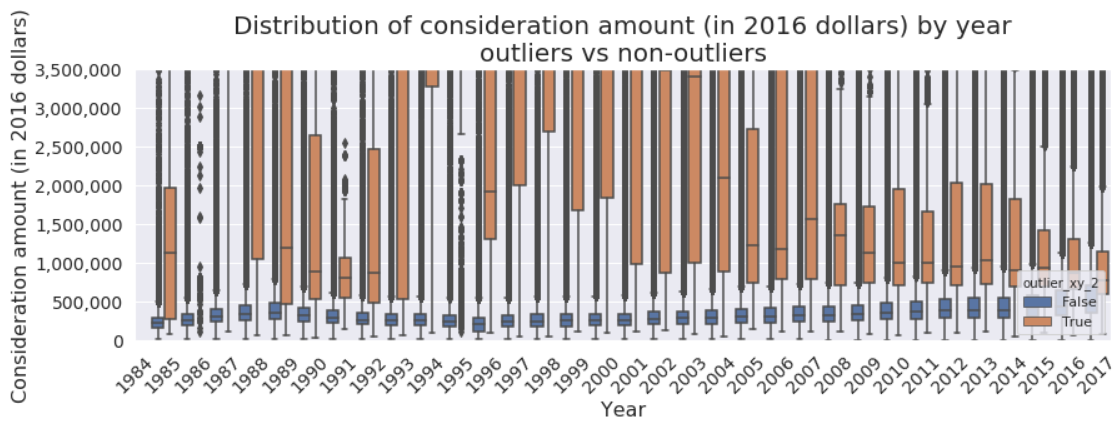
\includegraphics[width=.8\linewidth]{outliers_strict.png}
        \label{fig:top_outliers_mild}
        \caption{Outlier is 2 x median for 'xy'}
    \end{subfigure}

    \begin{subfigure}{\linewidth}
        \centering
        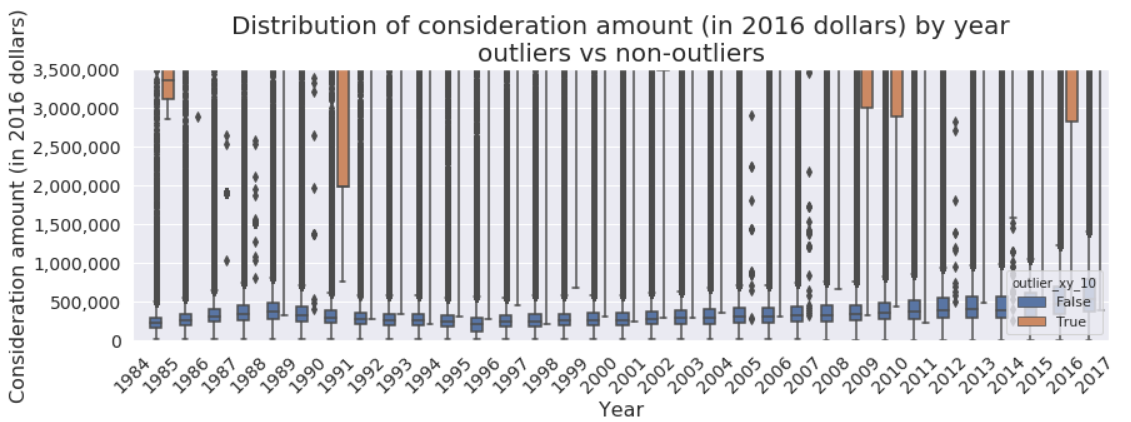
\includegraphics[width=.8\linewidth]{outliers_mild.png}
        \label{fig:top_outliers_strict}
        \caption{Outlier is 10 x median for 'xy'}
    \end{subfigure}
    \caption{Outliers at the high end of the price distribution most likely represent commercial, industrial and transactions of whole residential buildings.
    Since these transactions can still be useful for analysis, they are kept in the dataset and instead are marked using 7 new Boolean attributes representing criteria of varying strictness to define an outlier.
    The top subfigure presents an example where all transactions with price over 2 times greater than the median price for that 'xy' are considered to be an outlier, the bottom subfigure shows an example where only records with price over 10 times greater than median for 'xy' are marked as outliers.
    7 different criteria were used in total to mark top outliers.}
    \label{fig:top_outliers}
\end{figure}

For example, feature 'outlier\_y\_10' is a Boolean variable capturing if the price of a record, corrected for inflation, is over 10 times greater than the median price of all records for the corresponding year.
New attributes identifying outliers from the high end of the distribution in layers are added to each Teranet record and are used as features by the classification algorithm.

\section{Engineering new features for the classification algorithm} \label{sec:feature_engineering}

In addition to producing new keys for joining datasets, a number of new features is engineered from Teranet records to be tested with the classification algorithm (discussed in chapter~\ref{ch:ml_workflow}).
The new features are intended to give each Teranet transaction spatial and temporal "context" of the housing market dynamics by grouping Teranet records using various criteria.
For example, a feature 'xy\_prev\_sales' was added capturing the rolling count of Teranet records coming from this coordinate pair;
feature 'price\_to\_med\_year' captures a ratio of consideration amount of the current record to median consideration amount of all Teranet records for the corresponding year, etc.

The following features have been added to each Teranet record from 1985 to 2017 ('xy' represents 'x' and 'y' coordinates concatenated together as strings, used to group together all records coming from the same coordinate pairs):

\begin{itemize}
    \item 'price\_2016': consideration amount corrected for inflation using the coefficients from the Inflation Calculator provided by the Bank of Canada\cite{BankofCanada2019}
    \item 'pin\_total\_sales': count of Teranet records grouped by 'pin'
    \item 'xy\_total\_sales': count of Teranet records grouped by 'xy'
    \item 'pin\_prev\_sales': rolling count of Teranet records grouped by 'pin'
    \item 'xy\_prev\_sales': rolling count of Teranet records grouped by 'xy'
    \item 'xy\_first\_sale': a Boolean variable indicating whether it is the first record coming from this 'xy'
    \item 'pin\_years\_since\_last\_sale': difference in years since last record from this 'pin'
    \item 'xy\_years\_since\_last\_sale': difference in years since last record from this 'xy'
    \item 'xy\_years\_to\_next\_sale': difference in years to next record from this 'xy'
    \item 'da\_days/years\_since\_last\_sale': difference in days/years since last sale that occurred on this Dissemination Area
    \item 'xy\_sale\_next\_6m': a Boolean variable indicating whether there will be another sale on this 'xy' in the upcoming 6 month
    \item 'pin\_price\_cum\_sum': cumulative sum of inflation corrected price of all Teranet records from this 'pin'
    \item 'xy\_price\_cum\_sum': cumulative sum of inflation corrected price of all Teranet records from this 'xy'
    \item 'pin\_price\_pct\_change': percentage change of price corrected for inflation from the last Teranet record from this 'pin'
    \item 'xy\_price\_pct\_change': percentage change of price corrected for inflation from the last Teranet record from this 'xy'
    \item 'price\_da\_pct\_change': percentage change of price corrected for inflation from the last Teranet record from this Dissemination Area
    \item 'med\_price\_xy': median price corrected for inflation for all Teranet records from this 'xy'
    \item 'med\_price\_year': median price corrected for inflation for all Teranet records for this year
    \item 'price\_to\_med\_xy': ratio of price corrected for inflation to median price of all records for this 'xy'
    \item 'price\_to\_med\_year': ratio of price corrected for inflation to median price of all records for this year
    \item 'outlier\_y\_3': a Boolean variable marking as outliers all records with price more than 3 times greater than median for that year
    \item 'outlier\_y\_5': a Boolean variable marking as outliers all records with price more than 5 times greater than median for that year
    \item 'outlier\_y\_10': a Boolean variable marking as outliers all records with price more than 10 times greater than median for that year
    \item 'outlier\_y\_20': a Boolean variable marking as outliers all records with price more than 20 times greater than median for that year
    \item 'outlier\_xy\_2': a Boolean variable marking as outliers all records with price more than 2 times greater than median for that 'xy'
    \item 'outlier\_xy\_4': a Boolean variable marking as outliers all records with price more than 4 times greater than median for that 'xy'
    \item 'outlier\_xy\_10': a Boolean variable marking as outliers all records with price more than 10 times greater than median for that 'xy'
\end{itemize}

These new features were combined with TTS and Census variables via spatial and temporal relationships that were introduced in chapter~\ref{ch:spatial_and_temporal_relationships} and were used to train and test a classification algorithm to classify land use at Teranet transaction level, which will be described in chapter~\ref{ch:ml_workflow}.

\section{Chapter summary} \label{sec:data_preparation_summary}

The principles of ''Tidy data'', closely related to Codd's principles of database normalization, formalize the way how a shape of the data can be described and what goal should be pursued when formatting data.
The ''tidy data standard''  facilitates initial exploration and analysis of the data and simplifies the development of data analysis tools that work well together.
The structure of Teranet's dataset conforms with the ''Tidy data'' format.
Contrary to Teranet, tables with combined selected Census and TTS variables had variables for different Census and TTS years recorded as columns and thus needed to be ''melted''.
A new attribute 'year' was introduced to these tables to be used as a part of a composite foreign key when joining with Teranet records.

New foreign keys representing spatial identifiers, such as 'dauid' and 'taz\_o', were added to Teranet records via a series of spatial joins.
During the first join with Dissemination Area geometry used by Census, Teranet records with coordinates falling outside of GTHA have been filtered out.
Furthermore, Teranet records with consideration amount under 10'000 CAD were considered to be outliers at the low end of price distribution and were removed from the dataset.
Outliers at the high end of the price distribution were not removed, but instead were marked through 7 new Boolean attributes using various criteria to define a top outlier.
Finally, new features have been engineered to be tested with classification algorithms in chapter~\ref{ch:ml_workflow}.

\vspace{5mm}

Characteristics of the raw Teranet dataset:
\begin{itemize}
    \item 9,039,241 rows
    \item 15 columns
\end{itemize}

Characteristics of the Teranet dataset after data preparation described in this chapter:
\begin{itemize}
    \item 5,188,513 rows
    \item 75 columns
\end{itemize}

\chapter{A prototype of a machine learning workflow to classify land use} \label{ch:ml_workflow}

The fourth phase of CRISP-DM process model for data mining projects is modeling;
this chapter introduces a prototype of a machine learning workflow to classify land use from the housing market dynamics using the augmented Teranet dataset, production of which was described in chapter~\ref{ch:data_preparation}.
As was previously mentioned in section~\ref{sec:teranet_challenges_solution}, one of the major features missing from the available version of Teranet's dataset is the information about the type of property being transacted, which introduces a major limitation on how Teranet's data can be used.
As was described in chapter~\ref{ch:data_preparation}, parcel-level land use information from DMTI and the Department of Geography has been spatially joined to Teranet records, but these sources of land use information also have their limitations:

\begin{itemize}
    \item DMTI's land use data does not offer any split between subcategories of residential properties and only covers the period from 2001 to 2014
    \item land use data from the Department of Geography is a lot more detailed and accurate, but has been collected at a single point in time over the summer of 2012 and 2013
    \item neither of the available land use sources covers the full span of the Longitudinal Housing Market Research conducted by UTTRI (1986--2016)
\end{itemize}

To address this issue, detailed land use from the Department of Geography can be used as labelled data to train a machine learning model capable of recognizing certain property types that have characteristically different behavior on the housing market.
For example, the proposed model would be able to differentiate a detached house from a condo through such features as high / low volume of transactions, ratio of price to median price for that year, etc.
Chapter~\ref{ch:data_preparation} described the production of a dataset that combines the new features engineered from Teranet data with Census and TTS variables based on spatial and temporal relationships that were discussed in chapter~\ref{ch:spatial_and_temporal_relationships}.
In this chapter, this dataset is used to investigate the opportunity to implement a classification algorithm to determine the parcel land use at Teranet transaction level based on the housing market dynamics (land use is determined for each Teranet record, recognizing the changes of land use on the same parcel with time).
This way, a machine learning algorithm could provide a scalable solution to automate a labour-intensive task of collecting parcel-level detailed land use and expand the temporal span for which the land use data collected by Department of Geography can be used with accuracy.

\section{Selecting and encoding the target variable} \label{sec:select_encode_target}

According to the results of Exploratory Data Analysis (EDA), different property types have characteristically different behaviour on the housing market.
Figure~\ref{fig:xy_total_sales_dist_by_lu} shows the distributions of total count of Teranet records per coordinate pair by 10 most frequently encountered land use categories used in the Department of Geography's dataset.

\begin{figure}[hbt!]
    \centering
    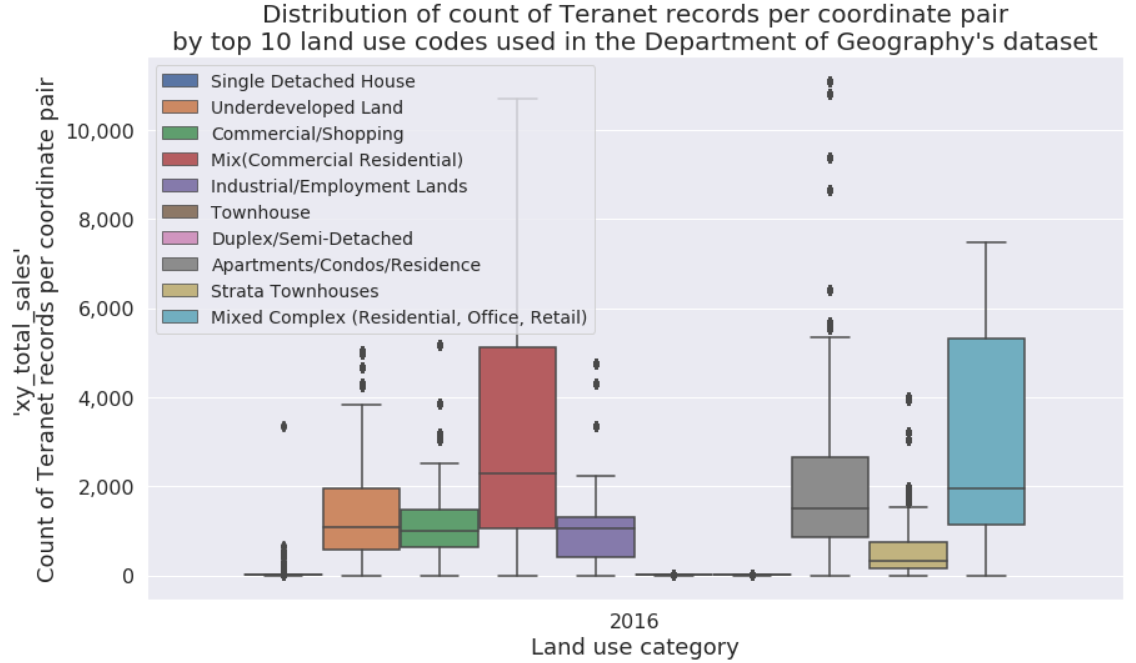
\includegraphics[width=0.98\linewidth,trim=0 0 0 0,clip]{xy_total_sales_dist_by_lu.png}
    \caption{Distributions of total count of Teranet records per coordinate pair by the top 10 land use categories.
    It can be seen that detached houses, duplexes, and townhouses ("collapsed" boxplots) have much lower number of records per coordinate pair.
    It can also be seen that there are some outliers present on the category of detached houses (first boxplot from the left).
    These outliers most likely represent mislabelled records, as it is very unlikely that a detached house can have almost 4'000 sales.}
    \label{fig:xy_total_sales_dist_by_lu}
\end{figure}

The target variable used for the purposes of investigating the possibility of land use classification using the housing market dynamics was constructed by reducing the land use codes found in the Department of Geography's land use dataset.
Department of Geography's land use categories that have the highest counts of Teranet records have been used to reduce all different property types to the three major land use classes.
Many machine learning algorithms are subject to a frequency bias in which they place more emphasis on learning from data observations which occur more frequently;
to address this, the three classes were selected to have a comparable number of Teranet records between themselves and thus produce a more balanced dataset.
In addition, chosen groupings combine categories that have a similar distribution of price and count of sales per coordinate pair between land use categories that were grouped together to form a single class.
For example, detached and semi-detached houses and townhouses would have a much smaller frequency of transaction and a higher median price per coordinate pair when compared to condos and strata townhouses.
Figure~\ref{fig:class_2_price_dist} shows an example of such grouping: for target class 1, Duplex/Semi-Detached properties are grouped together with Townhouses;
together with Single Detached Houses the three categories form a single target class ''house''.

\vspace{5mm}

The three target classes that were introduced are:

\begin{itemize}
    \item Class 0: "condo", including Apartments/Condos/Residence and Strata Townhouses
    \item Class 1: "house", including Single Detached Houses, Duplex/Semi-Detached and Townhouses
    \item Class 2: "other", including Commercial/Shopping, Mix (Commercial Residential), Industrial/Employment Lands, and everything else
\end{itemize}

\begin{figure}[ht]
    \centering
    \begin{subfigure}{\linewidth}
        \centering
        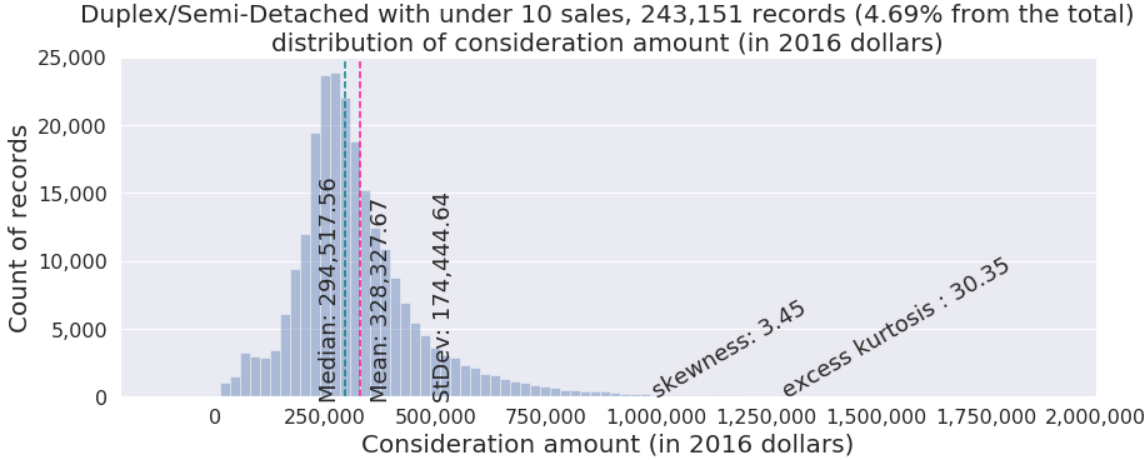
\includegraphics[width=.9\linewidth]{duplex_price_dist.png}
        \label{fig:duplex_price_dist}
        \caption{Duplex/Semi-Detached}
    \end{subfigure}

    \begin{subfigure}{\linewidth}
        \centering
        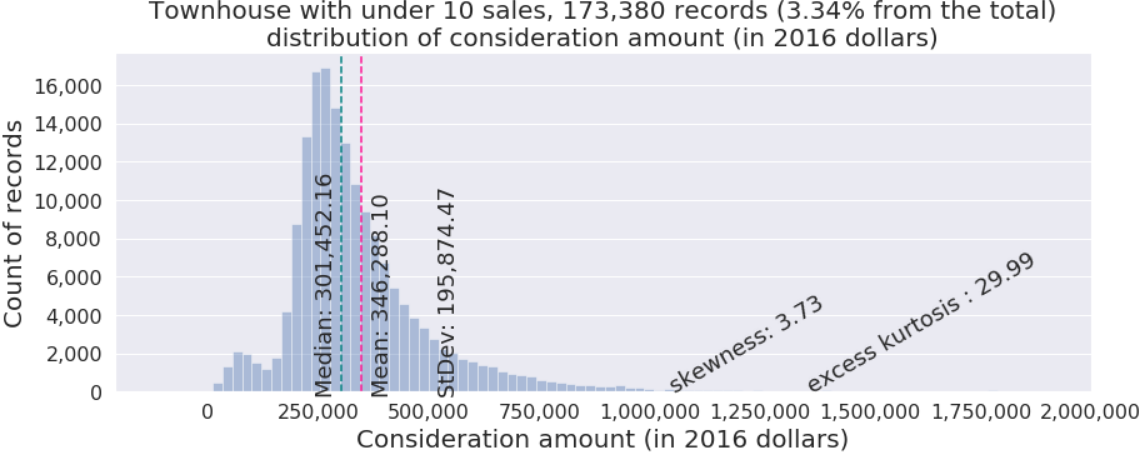
\includegraphics[width=.9\linewidth]{townhouse_price_dist.png}
        \label{fig:townhouse_price_dist}
        \caption{Townhouse}
    \end{subfigure}
    \caption{Distribution of price (in 2016 dollars) for two out of the three property types that are grouped together under Class 1: ''house''.
    Both categories have similar distributions of price and records per coordinate pair between themselves and with Single Detached Houses, and thus all three categories are grouped together to form a single target class ''house''.}
    \label{fig:class_2_price_dist}
\end{figure}

Classification algorithms, a subcategory of algorithms for supervised learning, predict the discrete unordered categorical class labels of new instances based on past observations.
A trained algorithm is capable of using a set of rules that were learned from past observations to distinguish the new instances between the possible classes.
Once the classes have been determined and assigned, the target variable must be encoded, as it is considered good practice to provide class labels as integer arrays to algorithms to avoid technical glitches and improve computational efficiency.
Class labels are not ordinal and classification estimators in scikit-learn\cite{scikit-learn} machine learning library in Python treat them as categorical data that does not imply any order.

\section{Missing values} \label{sec:missing_values}

As was mentioned in section~\ref{sec:feature_engineering}, some of the new features engineered from Teranet attributes, such as 'xy\_years\_since\_last\_sale' and 'xy\_years\_to\_next\_sale' contain missing values in each case of the first or the last Teranet record coming from a coordinate pair.
Since classification algorithms cannot handle inputs with missing values, during classification these values were replaced using the following logic:

\begin{itemize}
    \item For all the records with missing 'xy\_years\_since\_last\_sale' (first record from a coordinate pair), values were replaced with the median 'xy\_years\_to\_next\_sale' for this subset (median time interval in years between all future sales from this Teranet subset).
    \item For all the records with missing 'xy\_years\_to\_next\_sale' (last record from a coordinate pair), values were replaced with the median 'xy\_years\_since\_last\_sale' for this subset (median time interval in years between all past sales from this Teranet subset).
\end{itemize}

This replacement affects a large number of Teranet records, as there are many coordinate pairs with a low count of transactions in the dataset.
At the same time, it allows the classification algorithm to work on the majority of Teranet data, which improves the generalization of the algorithm and allows classifying land use of most Teranet records.
As will be discussed in chapter~\ref{ch:model_evaluation}, features that have missing values also have strong predictive power for land use classes and thus are best kept in the input set with the missing values replaced.
This replacement is done during the fitting of classification algorithm and is not recorded in the final version of Teranet's dataset with new features and keys, were the missing values are left as missing.

\section{Dimensionality reduction} \label{sec:dimensionality_reduction}

Quality of the data plays a critical part in the success of application of a machine learning algorithm, and one of important aspects of data quality is the dimensionality of input space.
The input space may contain features that are either redundant or irrelevant;
highly correlated features also introduce multicollinearity and can make the model unstable, or too sensitive to small changes in the input data.
In machine learning, statistics, and information theory, dimensionality reduction is the process of reducing the number of random variables under consideration;
there is a number of reasons for reducing dimensionality of a dataset:

\begin{enumerate}
    \item reducing the number of features improves computational efficiency and reduces training times
    \item in case of a low signal-to-noise ratio in the dataset, dimensionality reduction can improve the predictive performance of an algorithm\cite{RaschkaMirjalili2017}
    \item simpler models are easier to interpret\cite{James2013}
    \item excessive complexity of the model could cause overfitting\cite{RaschkaMirjalili2017}
    \item the curse of dimensionality\cite{Bellman1954} (in the context of machine learning, the curse of dimensionality describes the phenomena where the feature space becomes too sparse for the size of the training dataset)\cite{RaschkaMirjalili2017}
\end{enumerate}

There is a number of approaches that could be utilized to reduce the dimensionality of the feature space.
There are two main categories of dimensionality reduction techniques:
\begin{itemize}
    \item feature selection, also referred to as Feature Subset Selection, or (FSS), where a subset of the original features is selected
    \item feature extraction, where a new feature subspace is constructed from information derived from the original feature set
\end{itemize}

Feature selection can either be performed manually or by utilizing a feature selection algorithm.
Exhaustive evaluation of all possible feature subsets is computationally unfeasible even for a moderate number of features.
For example, if we are given a feature set with $m = 64$ features and want to reduce it to $n = 11$, an exhaustive evaluation would involve over $10^{11}$ possible feature subsets:

\begin{equation}
    _{m}C_n = _{64}C_{11} = \binom{64} {11} = \frac{64!} {11!(64 - 11)!} = 743,595,781,824
\end{equation}

Feature selection algorithms present a practical approach to feature selection at scale;
such algorithms combine a search strategy for proposing new feature subsets with an objective function to evaluate these subsets;
objective function plays the role of a feedback signal used by the search strategy to choose between candidate subset.
Objective functions are divided into three major groups:

\begin{itemize}
    \item filters
    \begin{itemize}
        \item evaluate candidate feature subsets by their information content (e.g., inter/intra class distance, mutual information, etc.)
        \item advantages: have faster execution time since there generally is no iterative computation;
        have good generality since they evaluate the intrinsic properties of the data.
        \item disadvantages: tend to select large feature subsets due to monotonic objective functions
    \end{itemize}
    \item wrappers
    \begin{itemize}
        \item use a classifier to evaluate subsets by their predictive accuracy
        \item advantages: have better accuracy since they select subsets based on specific interactions between the classifier and the dataset
        \item disadvantages: slower to execute since a classifier needs to be re-trained multiple times;
        selected feature subset will be specific to the classifier that was used to evaluate the candidate subsets.
    \end{itemize}
    \item embedded methods
    \begin{itemize}
        \item feature selection is performed as a part of model construction process (i.e., LASSO method for constructing a linear model with L1 regularization)\cite{Scikit-learndevelopers2019}
    \end{itemize}
\end{itemize}

A combination of different FSS techniques was applied to reduce the dimensionality of the dataset with Teranet, TTS, and Census variables for classification from 64 to 11 input features.
The first method utilized was SelectFromModel in scikit-learn, a wrapper FSS algorithm that selects an optimal size and composition of a feature subset by fitting the provided classifier to training data and getting the importance weights from the fit model.
SelectFromModel with Random Forest classifier has determined the optimal number of features to be 18;
this number of features was provided to the other FSS algorithms to select the 18 best features from the dataset according to each method.

The second FSS method that was applied to the augmented Teranet dataset comes from the filter family of objective functions: a univariate feature selection algorithm SelectKBest in scikit-learn;
this method selects $k$ highest scoring features based on their scores on the specified univariate statistical test.
Univariate FSS techniques can be useful for better understanding of the data, as they examine each feature individually to determine the strength of its relationship with the target variable.
However, due to this fact, these methods will not necessarily result in improvement in the generalization of a learning algorithm, and thus their results have been used for feature selection in combination with other methods discussed in this section.
The following statistical tests from scikit-learn have been selected for scoring features using SelectKBest FSS algorithm:

\begin{itemize}
    \item Chi-squared stats of non-negative (pre-normalized) features for classification tasks
    \item ANOVA F-value between label/feature for classification tasks
    \item Mutual information for a discrete target
\end{itemize}

The third family of FSS algorithms that were applied were the recursive feature elimination algorithms, wrapper algorithms that evaluate candidate feature subsets and recursively eliminate features until the desired number of dimensions is reached.
RFE class in scikit-learn facilitates feature ranking with recursive feature elimination using the provided external classifier that assigns weights to features.
A more exhaustive approach to recursive feature elimination is the use of a sequential feature selection algorithm.
Sequential feature selection algorithms are a family of greedy search algorithms that are used to reduce an initial $d$-dimensional feature space to a $k$-dimensional feature subspace where $k<d$.

\begin{figure}[hbt!]
    \centering
    \begin{subfigure}[t]{.45\textwidth}
        \centering
        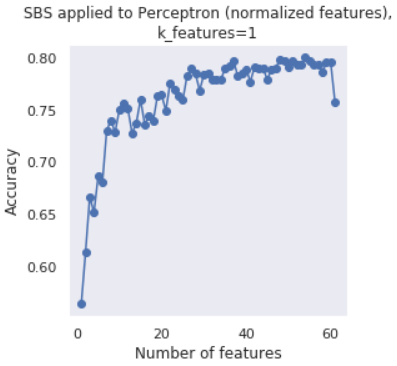
\includegraphics[width=\columnwidth,trim=0 0 0 0,clip]{sbs_perceptron.png}
        \caption{Perceptron}
        \label{fig:sbs_perceptron}
    \end{subfigure}
    ~ %add desired spacing between images, e. g. ~, \quad, \qquad, \hfill etc.
    %(or a blank line to force the subfigure onto a new line)
    \begin{subfigure}[t]{.53\textwidth}
        \centering
        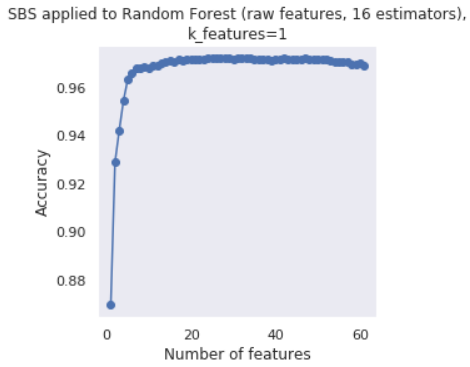
\includegraphics[width=\columnwidth,trim=0 0 0 0,clip]{sbs_forest.png}
        \caption{Random Forest}
        \label{fig:sbs_forest}
    \end{subfigure}
    \caption{Sequential Backward Selection (SBS) is a classic sequential FSS algorithm;
    on each iteration, it eliminates the feature that results in the minimum drop in performance of the provided classifier.
    Figure~\ref{fig:sbs_perceptron} shows SBS run on augmented Teranet dataset with Perceptron and figure~\ref{fig:sbs_forest} shows SBS with Random Forest.
    It can be seen that many features can be eliminated without a significant drop in performance of both classifiers, especially in the case of Random Forest.}
    \label{fig:sbs_teranet}
\end{figure}

Sequential Backward Selection (SBS) is a classic sequential FSS algorithm which aims to reduce the dimensionality of the initial feature subspace with a minimum decay in performance of the classifier;
in some cases of model overfitting, SBS can even improve the predictive power of a classifier.
On each iteration, a feature is removed using the defined criterion function $J$ that we want to minimize;
$J$ can simply be defined as the difference in performance of the classifier before and after the elimination of a particular feature.
Figure~\ref{fig:sbs_teranet} presents plots produced by running SBS algorithm on augmented Teranet dataset with Perceptron and Random Forest;
Sequential Backward Selection algorithm implemented as a Python class by Raschka and Mirjalili\cite{RaschkaMirjalili2017} has been used for this master's thesis.

\begin{figure}[hbt!]
    \centering
    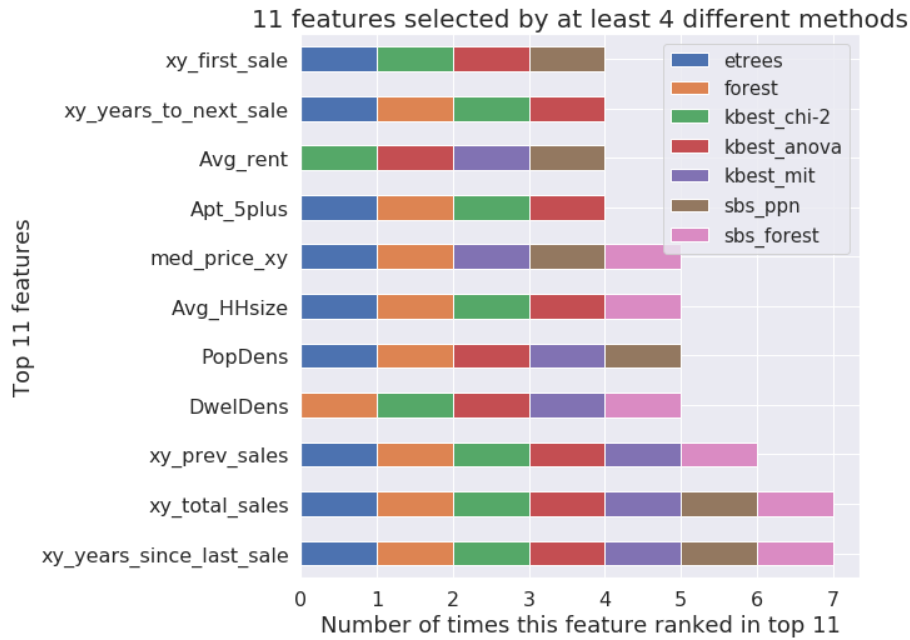
\includegraphics[width=0.7\linewidth,trim=0 0 0 0,clip]{top11f_selection_summary.png}
    \caption{FSS results: 11 features that were selected by at least four different feature selection methods.
    These features were used to select the best-performing model and make the final classification of land use of Teranet records.}
    \label{fig:top_feats}
\end{figure}

As can be seen from the plots produced by SBS, most features in the augmented Teranet dataset can be eliminated without a significant drop in performance of both linear and tree-based models.
As such, final set of features to be used for land use classification was selected by combining the feature subsets selected by each of the FSS methods described above.
Features that have been selected by at least four different methods were selected as the final feature subset that was tested with the classification algorithms and used for final classification of land use;
figure~\ref{fig:top_feats} presents the 11 features that were selected using this logic: these are the 11 features that were selected by at least four different FSS techniques.

From the perspective of embedded feature selection methods, another possible approach to reduce the complexity of a model is to use L1 regularization to penalize large individual weights.
L1 regularization introduces a penalty term to the cost function which is taken as the norm of the weight vector defined as:

\begin{equation} \label{eq:l1_regularization}
    L1:~\norm{\vect{w}}_1 = \sum \limits_{j=1}^m \abs{w_j}
\end{equation}

L1 regularization is similar to L2 regularization, which is defined as:

\begin{equation} \label{eq:l2_regularization}
    L2:~\norm{\vect{w}}_2^2 = \sum \limits_{j=1}^m w_j^2
\end{equation}
where $m$ is the number of features.

However, since in the case of L1 regularization, the sum of squares of weights is replaced with the sum of the absolute values of weights, L1 regularization usually yields sparse feature vectors, since most feature weights will be zero\cite{RaschkaMirjalili2017,Scikit-learndevelopers2019}.
Sparsity of feature vectors can help us get rid of irrelevant features in a high-dimensional dataset;
in this context, L1 regularization can be understood as a technique for feature selection\cite{RaschkaMirjalili2017}.
L1 regularization was attempted with Logistic Regression and Linear Support Vector Classifier models in scikit-learn, but did not result in a significant improvement in model performance.

\section{Tuning model hyperparameters} \label{sec:tuning_hyperparameters}

One of the critical aspects of evaluating the performance of a machine learning model is the assessment of algorithm's ability to not only perform well on the data that was used to train it, but also to generalize well to unseen, or test, data;
comparing predictions made by the algorithm to true labels in the test subset can be understood as the unbiased performance evaluation of the model\cite{RaschkaMirjalili2017}.
To facilitate this, all GTHA Teranet records from 2011 to 2014 have been randomly split into two subsets: 70\% of the data was used to train models and tune their hyperparameters, while 30\% of the data has been used as a test subset for unbiased performance evaluation of the classifier.
Train and test subsets have been stratified across the target classes:
in this context, stratification means that training and test subsets will have the same proportions of class labels as the input dataset.

\begin{figure}[hbt!]
    \centering
    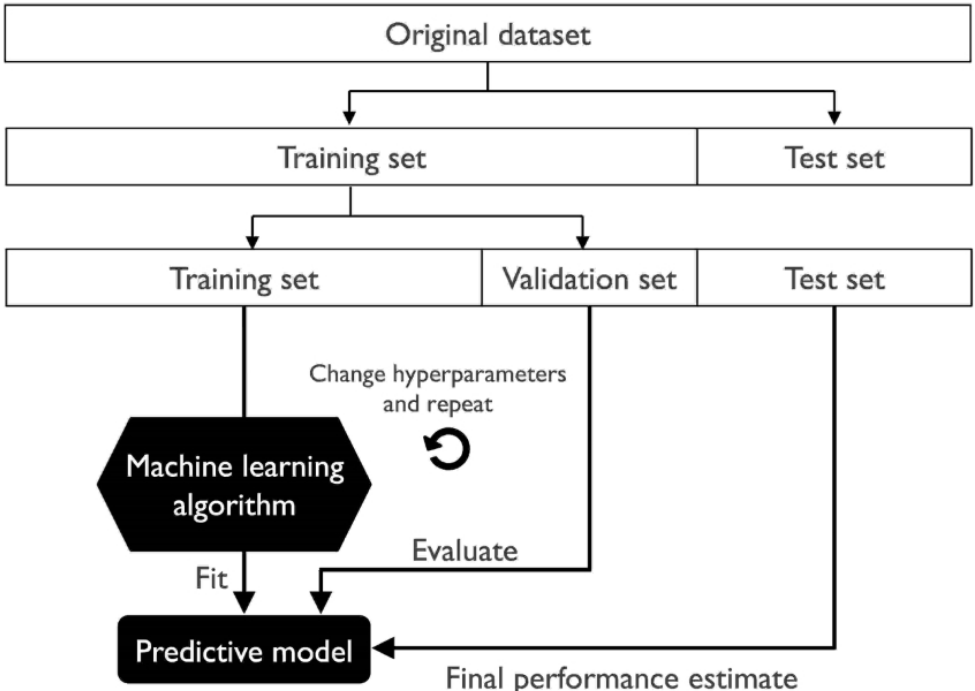
\includegraphics[width=0.7\linewidth,trim=0 0 0 0,clip]{holdout_validation_workflow.png}
    \caption{Holdout validation of a machine learning model as summarized by Raschka and Mirjalili\cite{RaschkaMirjalili2017}.}
    \label{fig:holdout_validation_workflow}
\end{figure}

There are two types of parameters in machine learning: those that are learned by parametric models from training data (i.e., wights in logistic regression), and the parameters that tune the performance of a learning algorithm, or its hyperparameters (i.e., regularization parameter in logistic regression or maximum depth of a decision tree).
If a model is too simple, it can suffer from underfitting and show poor performance on both the training and the test data (have high bias);
on the other hand, if it is too complex, it can overfit the training data and have poor generalization on test data (have high variance).
An acceptable bias-variance trade-off can be found by tuning the hyperparameters of a learning model, but care must be taken to ensure unbiased assessment of its generalization performance.

When evaluating different hyperparameters for estimators, there is a risk of overfitting on the test set because knowledge about the test set can ''leak'' into the model;
evaluation metrics will no longer report on generalization performance.
To address this issue, yet another part of the dataset can be held out as a so-called ''validation set'': training proceeds on the training set, with model hyperparameters being evaluated by its performance on the validation set;
when the experiment seems to be successful, final evaluation can be done on the test set.
Figure~\ref{fig:holdout_validation_workflow} presents an example of a workflow for tuning and evaluating a machine learning model using hold-out validation, as summarized by Raschka and Mirjalili\cite{RaschkaMirjalili2017}.

\begin{figure}[hbt!]
    \centering
    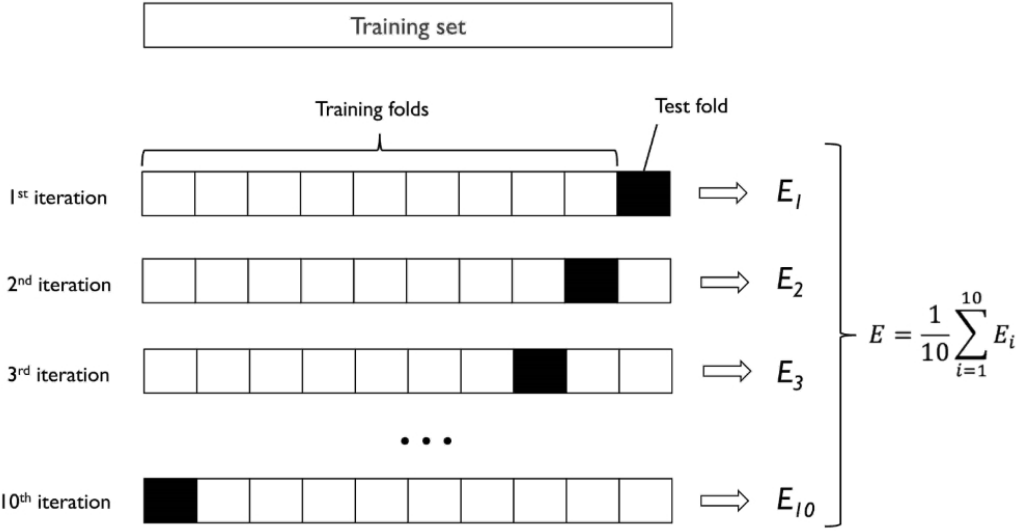
\includegraphics[width=0.9\linewidth,trim=0 0 0 0,clip]{kfold_validation_workflow.png}
    \caption{$k$-fold cross-validation as summarized by Raschka and Mirjalili\cite{RaschkaMirjalili2017}.
    In the case of $k=10$, the training dataset is divided into 10 folds, and during the 10 iterations, nine folds are used for training, and one fold is used as the test set for the model evaluation.
    Estimated performances (for example, classification accuracy or error) for each fold are then used to calculate the estimated average performance $E$ of the model.}
    \label{fig:kfold_validation_workflow}
\end{figure}

There is a shortcoming in this approach: by partitioning the available data into three sets, the number of samples which can be used for learning the model is drastically reduced;
results can depend on a particular random choice of the train and validation sets.
A solution to this problem is a procedure called cross-validation (CV for short): validation set is produced from the training set using such techniques as $k$-fold CV, while the test subset of data unseen by the model is held out for its final evaluation.
In a basic approach called $k$-fold CV, the training set is split into $k$ smaller sets and on each of $k$ iterations a model is trained using $k-1$ of the folds as training data;
the resulting model is validated on the held-out test fold of the data through such performance metrics as model accuracy.
The performance measure reported by $k$-fold cross-validation is then the average of the values computed in the loop.
Figure~\ref{fig:kfold_validation_workflow} presents $k$-fold cross-validation workflow to evaluate model performance as summarized by Raschka and Mirjalili\cite{RaschkaMirjalili2017}.

This approach can be computationally expensive, but does not waste too much data, as is the case when fixing an arbitrary validation set.
Empirical evidence shows that a good standard value for $k$ in $k$-fold cross-validation is 10, as seen in experiments conducted by Kohavi on various real-world datasets\cite{Kohavi1995}.
A light further improvement in bias and variance estimates over the standard $k$-fold cross-validation can be achieved by using stratified $k$-fold cross-validation, as shown in the study conducted by Kohavi.
In stratified cross-validation, the class proportions are preserved in each fold to ensure that each fold is representative of the class proportions in the training dataset.
For this master's thesis, stratified $k$-fold cross-validation workflow has been used to tune model hyperparameters via grid search before the final evaluation of model performance was done using the held-out test set;
model evaluation results will be discussed in chapter~\ref{ch:model_evaluation}.

\section{Feature scaling} \label{sec:feature_scaling}

Many machine learning algorithms are designed with the assumption that each feature takes values close to zero or, more importantly, that all features vary on comparable scales\cite{Scikit-learndevelopers2019b}.
Raw data rarely comes in the form and shape that is necessary for the optimal performance of a learning algorithm, and thus data preprocessing via scaling is one of the most crucial steps in machine learning workflows\cite{RaschkaMirjalili2017}.
Bringing different variables on the same scale can be accomplished by such techniques as standardization or normalization;
in addition, outliers that are present in data can be addressed by using non-linear transformations, such as quantile or power transforms.

\vspace{5mm}

The following preprocessing methods have been tested on the training dataset:

\begin{itemize}
    \item standardization (mean removal and variance scaling)
    \item normalization (min-max scaling to a range of [0, 1])
    \item max-abs (scale to a range of [-1, 1], maximum absolute value of each feature is scaled to unit size)
    \item robust scaling (more robust estimates for data with outliers)
    \item power transform (Yeo-Johnson, mapping to a Gaussian distribution)
    \item quantile transform (mapping to a Gaussian distribution)
    \item quantile transform (mapping to a uniform distribution)
    \item sample-wise L2 transform (normalize samples individually to unit norm)
\end{itemize}

All these preprocessing techniques were tested with classification algorithms for prediction accuracy and fit times;
results will be presented in chapter~\ref{ch:model_evaluation}.
It is important to note that the parameters for the previously mentioned procedures, such as feature scaling and dimensionality reduction, are solely obtained from the training dataset, and the same parameters are later reapplied to transform the test dataset and the full Teranet dataset for the final classification of land use;
this way, an unbiased estimate of model generalization can be obtained.

\section{Model selection} \label{sec:model_selection}

An important point to be summarized from the famous No Free Lunch Theorems (NFL)\cite{Wolpert1996,Wolpert1997} by David H. Wolpert is that no single classifier works best across all possible scenarios, as there is a lack of a priori distinctions between learning algorithms.
In practice, it is essential to compare the performance of at least a handful of different classification algorithms, since each of them has its inherent biases, in order to select the best performing model.
No single classification model enjoys superiority if we don't make any assumptions about the form of the function that maps input features to target variables and how this function can be learned\cite{RaschkaMirjalili2017}.

There are several possible ways of categorizing machine learning algorithms;
one of them is to separate algorithms into parametric and non-parametric models.
In parametric models, such as logistic regression, perceptron or linear Support Vector Machine (SVM), model parameters are estimated from the training set to learn a function that allows classifying new data without the need for the original training set, once the model has been fit.
In addition, the number of model parameters is fixed and does not change with the size of the training data.
In contrast, non-parametric models, such as instance-based learning models like $k$-Nearest Neighbors, can't be characterized by a fixed set of parameters, and the number of parameters grows with the amount of training data.

Another way of categorizing the algorithms that were used in this master's thesis is into linear, tree-based, and nearest neighbors model classes.
Models from the following three main classes of classification algorithms have been tested with the augmented Teranet dataset:

\begin{itemize}
    \item Linear models

    Linear models are used by a popular and broad class of procedures for solving classification tasks.
    These models aim at dividing the feature space into a collection of regions labelled according to the values that the target can take, where the decision boundaries between those regions are linear hyperplanes.

    \begin{itemize}
        \item Perceptron learning algorithm

        Perceptron is a simple classification algorithm suitable for large-scale learning that was introduced by Frank Rosenblatt\cite{Rosenblatt1957a} in 1957 based on the McCulloch-Pitts (MCP) artificial neuron model\cite{McCulloch1990a} that was introduced in 1943.
        It is a parametric non-regularized model that only updates its weights on wrong predictions that it makes.

        \item Logistic Regression (L2, L1 regularization)

        Another simple yet more powerful parametric algorithm for linear and binary classification problems is logistic regression;
        it can also be expanded to multi-class problems through such techniques as One-versus-All (OvA).
        Logistic regression models the probabilities of an observation belonging to each of the $K$ classes via linear functions and is typically estimated by maximum likelihood.
        It is often used as an inference tool to understand the role of input variables in explaining the target, since it produces easily interpretable coefficients;
        in addition, it can also have significant predictive power in the cases when target classes are linearly separable\cite{RaschkaMirjalili2017}.

        \item Linear Discriminant Analysis

        Linear Discriminant Analysis (LDA) is most commonly used as a dimensionality reduction technique, but it can also have some practical uses as a classifier by itself.
        LDA assumes that the joint densities of all features given target's classes are multivariate Gaussians with the same covariance for each class.

        \item Quadratic Discriminant Analysis

        Quadratic Discriminant Analysis (QDA) is a classifier with a quadratic decision boundary;
        it relaxes the common covariance assumption of LDA through estimating a separate covariance matrix for each class.

        \item Linear Support Vector Classification (L2, L1 regularization)

        Support Vector Machines (SVM) represent another family of powerful and widely used algorithms used for maximum margin classification: optimization objectives for SVMs is to maximize the margin instead of minimizing the classification error.
        The margin is defined as the distance between the separating hyperplane (decision boundary) and the training samples that are closest to this hyperplane, which are the so-called support vectors\cite{RaschkaMirjalili2017}.

        \item Naive Bayes Classifier

        A Naive Bayes Classifier is a probabilistic classification technique based on Bayes Theorem with an assumption of independence among input features.
        It determines the probability that an example belongs to some class, calculating the probability that an event will occur given that some input event has occurred.
        These algorithms are computationally efficient and suitable for large datasets, but have the disadvantage of the assumption about the independence of input features.

    \end{itemize}

    \item Tree-based models

    Decision tree classifiers are attractive models due to their predictive power, computational efficiency and interpretability.
    In addition, these models are scale-invariant and require less data preprocessing.
    These models construct a flow-chart-like decision tree by learning simple decision rules similar to asking a series of questions.

    \begin{itemize}

        \item Decision Tree Classifier

        Decision trees can build complex decision boundaries by dividing the feature space into rectangles by learning a series of questions to infer the class labels of the samples;
        questions are selected to maximize Information Gain (IG) on each split of the tree, defined as the difference in selected impurity measure (Gini, entropy, or classification error) between parent and child nodes.
        Splitting procedure is repeated until all the leaves are pure (consist of samples belonging to the same target class), or until selected maximum depth of the tree is reached.

        \item Random Forest Classifier

        Since decision trees can be unstable due to small variations in the data, a more robust approach is to combine multiple trees into an ensemble model.
        Random forest is a hugely popular classification algorithm due to its good classification performance, scalability, and ease of use\cite{RaschkaMirjalili2017}.
        Random forest averages multiple (deep) decision trees each of which individually suffers from high variance, to build a model with better generalization performance and less susceptible to overfitting.
        Prediction of the class label is aggregated by a majority vote from the selected number of trees, each of which was trained on a bootstrapped sample using a randomly selected subset of features.

    \end{itemize}

    \item Nearest Neighbors


    Neighbors-based classification presents a type of instance-based non-parametric learning: it does not attempt to construct a discriminative function to classify the target variable;
    instead, it simply stores instances of the training data.
    The principle behind nearest neighbors is to find a predefined number of training samples closest in distance to the new point, and predict the target label of a new sample using the majority vote of its neighbors.
    The number of samples can either be a user-defined constant ($k$-nearest neighbor learning), or vary based on the local density of points (radius-based neighbor learning).
    Commonly used distance metrics include Manhattan and Euclidean distance.

    \begin{itemize}

        \item $k$-Nearest Neighbors Classifier

        $k$-Nearest Neighbors classifier is a distance-based classification algorithm that uses a predefined number of samples considered as neighbors to each new point according to the selected distance metrics (Manhattan, Euclidean distances are a common choice).
        Class label of each new point is assigned by the majority vote of its neighbors.
        Number of neighbors $k$ and distance metric are the hyperparameters of a $k$-NN model.

    \end{itemize}

\end{itemize}

In order to compare different models, metrics to measure performance needed to be established, which will be discussed in section~\ref{sec:model_metrics}.
Results of model evaluation are presented in chapter~\ref{ch:model_evaluation}.

\section{Chapter summary} \label{sec:ml_workflow_summary}

One of the major features missing from Teranet's dataset is land use information covering a period of time starting from 1985.
This chapter introduced a prototype of machine learning workflow to classify land use at Teranet transaction level from housing market dynamics as reflected by augmented Teranet variables.
Such topics as methodology for feature selection, filling of the missing values, feature scaling, model hyperparameter tuning, unbiased assessment of model performance via such techniques as train-test split and $k$-fold cross-validation and selection of learning algorithms to be tested have been discussed in this chapter.
Chapter~\ref{ch:model_evaluation} presents the evaluation of model performance.
\chapter{Model evaluation} \label{ch:model_evaluation}

\section{Metrics for evaluating model performance} \label{sec:model_metrics}

\section{Model performance} \label{sec:model_performance}

Model hyperparameters were tuned for each classifier using $k$-fold cross validation, as was described in section~\ref{sec:tuning_hyperparameters}.
After the tuning, performance of the following models have been compared:

\begin{itemize}
    \item Perceptron learning algorithm, learning rate $\eta=0.5$, maximum iterations=5, features transformed with quantile transformation (uniform PDF)

    model code: ppn\_qu\_eta0.5\_maxiter5

    \item Logistic regression, L2 regularization, regularization parameter $C=0.1$, maximum iterations=100, features transformed with quantile transformation (uniform PDF)

    model code: lr\_l2\_c0.1\_maxiter\_100

    \item Logistic regression, L1 regularization, regularization parameter $C=0.1$, maximum iterations=100, features transformed with quantile transformation (uniform PDF)

    model code: lr\_l1\_c0.1\_maxiter\_100

    \item Linear Discriminant Analysis, features transformed with quantile transformation (uniform PDF)

    model code: lda

    \item Quadratic Discriminant Analysis, features transformed with quantile transformation (uniform PDF)

    model code: qda

    \item Linear Support Vector Classification, L2 regularization, regularization parameter $C=0.1$, maximum iterations=100, features transformed with quantile transformation (uniform PDF)

    model code: lsvc\_l2\_c0.1\_maxiter\_100

    \item Linear Support Vector Classification, L1 regularization, regularization parameter $C=0.1$, maximum iterations=100, features transformed with quantile transformation (uniform PDF)

    model code: lsvc\_l1\_c0.1\_maxiter\_100

    \item Gaussian Naive Bayes

    model code: nb

    \item Decision Tree, Gini impurity criterion, maximum depth of the tree=25, unscaled features

    model code: tree25

    \item Random Forest, Gini impurity criterion, number of estimators=50, unscaled features

    model code: forest50

    \item K-Nearest Neighbors, Manhattan distance metric, number of neighbors=4, standardized features

    model code: knn\_p1\_k4
\end{itemize}

Four different subsets of data have been used to test the model: train, test, and two additional validation subsets.
The train and test subsets represent Teranet records from 2011 to 2014 randomly sampled into 70\% train and 30\% test subsets;
these are the primary subsets that were used for training and tuning the hyperparameters and then evaluating the performance of classifiers on unseen test data.
The two additional validation subsets are composed of Teranet records from 2010 and 2015.
Since the land use information from Department of Geography was collected in 2012 and 2013, it can be less accurate for these subsets;
these subsets have not been used for model training or selection, but are presented as an additional reference for the generalization of performance of classifiers.
Figure~\ref{fig:model_performance} presents model performance on train, test, and two additional validation subsets.

\begin{figure}[hbt!]
    \centering
    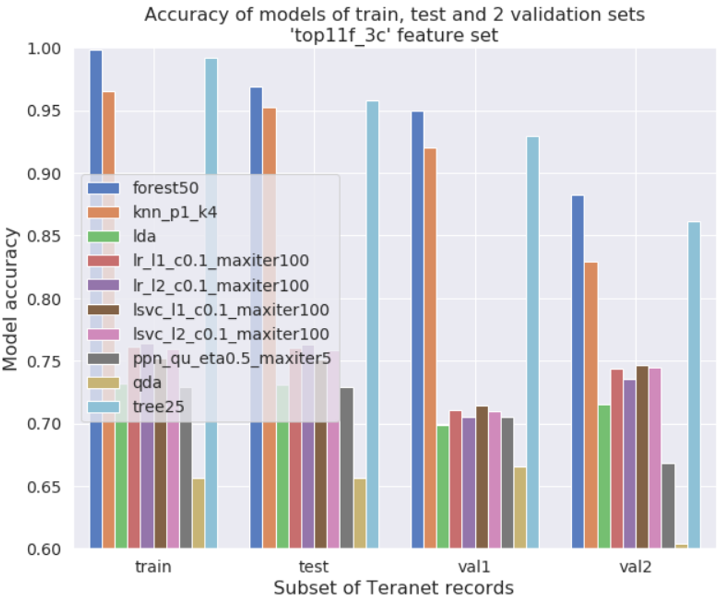
\includegraphics[width=0.6\linewidth,trim=0 0 0 0,clip]{model_performance.png}
    \caption{Model performance (accuracy) on train, test, and two additional validation subsets.
    Additional validation subsets are composed of Teranet records from 2010 and 2015;
    since land use information (target variable) can be less accurate for records in these subsets, they have been used as an additional reference for evaluating the generalization of the classifier performance.}
    \label{fig:model_performance}
\end{figure}

Different feature scaling techniques have a strong effect on model fit times and predictive performance of linear models, as can be seen on figure~\ref{fig:fit_times_linear}.

\begin{figure}[hbt!]
    \centering
    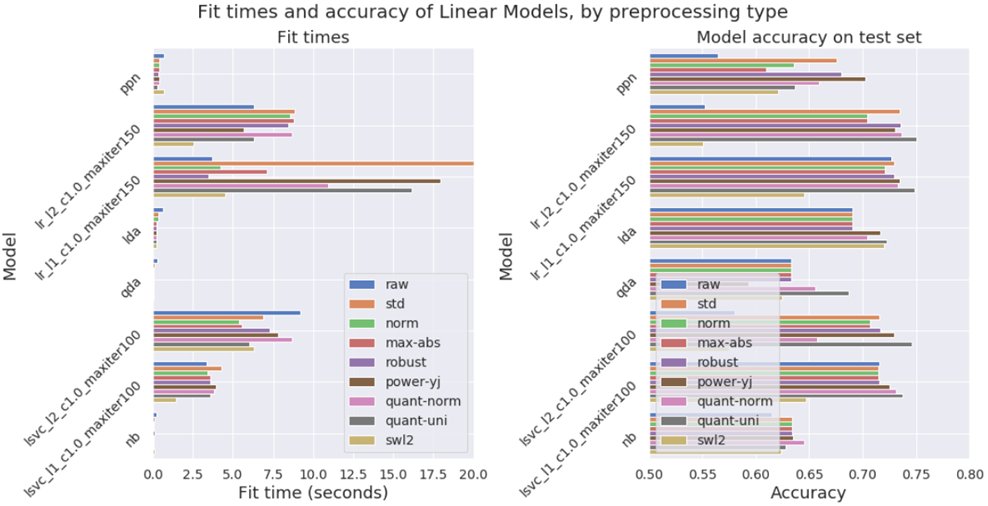
\includegraphics[width=0.98\linewidth,trim=0 0 0 0,clip]{fit_times_linear.png}
    \caption{Fit times and accuracy of linear models, by feature scaling technique.
    Different scaling techniques have a strong effect on the performance of linear models.}
    \label{fig:fit_times_linear}
\end{figure}

Similar to linear models, distance-based algorithms, such as K-Nearest Neighbors, also are strongly affected by feature scaling.
In contrast, tree-based models, such as Decision Tree and Random Forest, are scale-invariant, and thus have stable performance with most feature scaling techniques.
Figure~\ref{fig:fit_times_trees_neighbors} presents fit times for Decision Tree, Random Forest, and K-Nearest Neighbors with Manhattan and Euclidean distance metrics.


\begin{figure}[ht]
    \centering
    \begin{subfigure}{\linewidth}
        \centering
        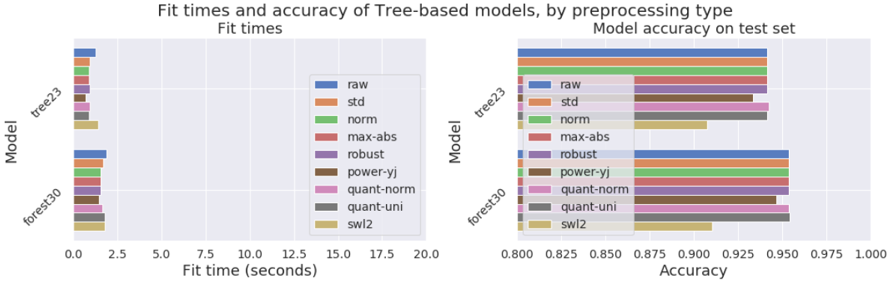
\includegraphics[width=.98\linewidth]{fit_times_trees.png}
        \label{fig:fit_times_trees}
        \caption{Tree-based models: Decision Tree and Random Forest}
    \end{subfigure}

    \begin{subfigure}{\linewidth}
        \centering
        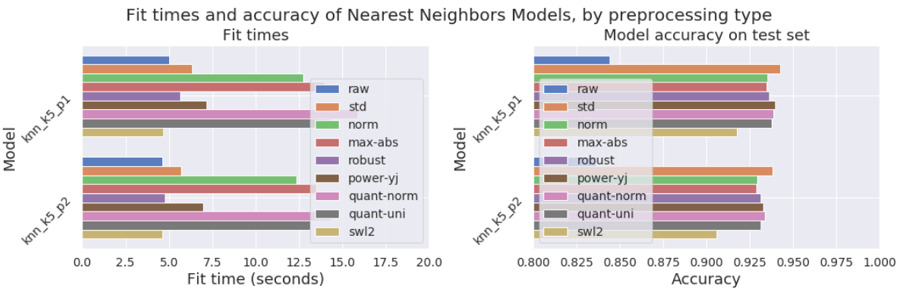
\includegraphics[width=.98\linewidth]{fit_times_neighbors.png}
        \label{fig:fit_times_neighbors}
        \caption{K-Nearest Neighbors: Manhattan and Euclidean distance}
    \end{subfigure}
    \caption{Fit times and accuracy for tree-based models and K-Nearest Neighbors, by feature scaling technique.
    Distance-based algorithms, such as K-Nearest Neighbors are affected by feature scaling, while tree-based models are scale-invariant.}
    \label{fig:fit_times_trees_neighbors}
\end{figure}

\section{Best performing model: Random Forest} \label{sec:best_performing_model}

Random Forest as can be seen from the plots presented in section~\ref{sec:model_performance}, Random Forest with 50 estimators and Gini impurity criterion showed the best results in terms of accuracy and fit times on all subsets.
Figure~\ref{fig:classification_report_train_test} presents the classification report showing all main model performance metrics for the best performing model: Random Forest with 50 estimators using 'gini' crietrion.

\begin{figure}[hbt!]
    \centering
    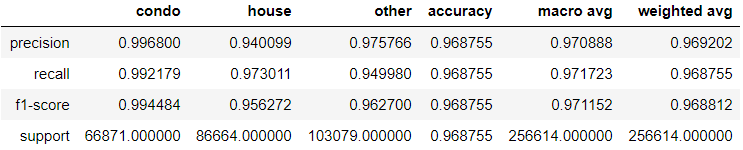
\includegraphics[width=0.98\linewidth,trim=0 0 0 0,clip]{classification_report_train_test.png}
    \caption{Best model performance on test set: classification report for Random Forest with 50 estimators using 'gini' criterion.}
    \label{fig:classification_report_train_test}
\end{figure}

Figure~\ref{fig:confusion_matrix_train_test} presents confusion matrices with and without normalization for Random Forest on the test set.

\begin{figure}[hbt!]
    \centering
    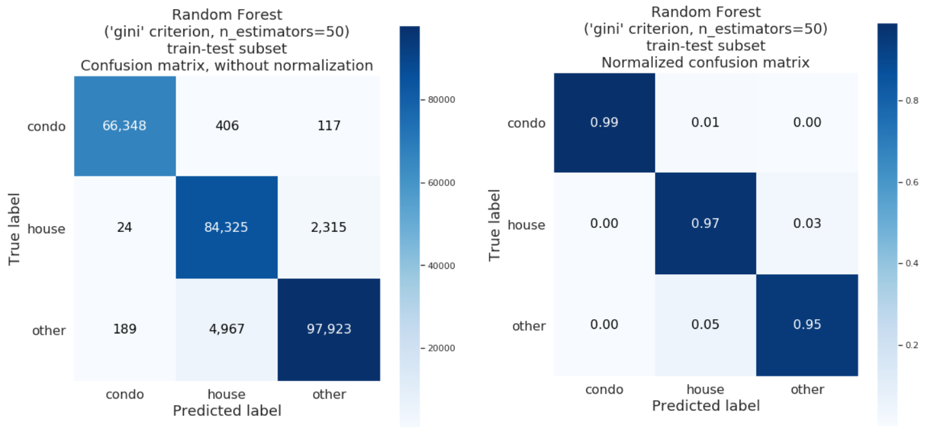
\includegraphics[width=0.98\linewidth,trim=0 0 0 0,clip]{confusion_matrix_train_test.png}
    \caption{Best model performance on test set: confusion matrices with and without normalization for Random Forest with 50 estimators using 'gini' criterion.}
    \label{fig:confusion_matrix_train_test}
\end{figure}

Figure~\ref{fig:forest_feature_importance} presents feature importance for the best performing model.

\begin{figure}[hbt!]
    \centering
    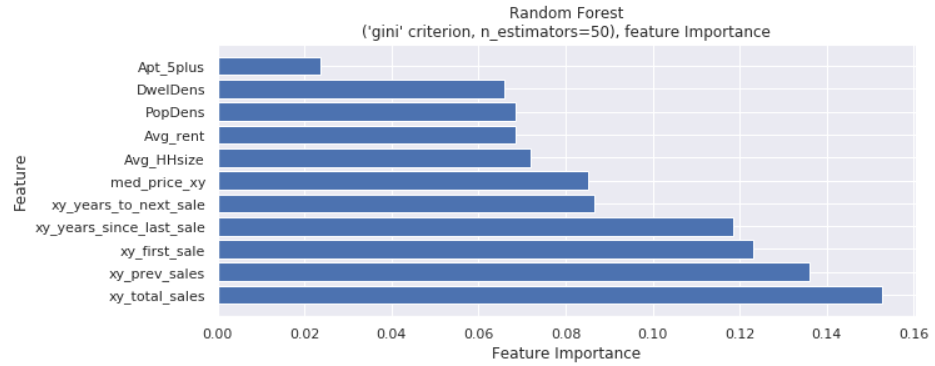
\includegraphics[width=0.98\linewidth,trim=0 0 0 0,clip]{forest_feature_importance.png}
    \caption{Random Forest with 50 estimators using 'gini' criterion: feature importance.}
    \label{fig:forest_feature_importance}
\end{figure}

\chapter{Conculsion} \label{ch:conclusion}

Microsimulation models present the latest generation of integrated land use and transportation models and are well suited to analyze the complex interaction of transportation and land use.
New data sources that appear with the increased digitization of human activity present opportunities to look at urban processes at unprecedented spatial and temporal scale, and thus present a lot of value for design and validation of integrated urban models and for longitudinal studies concerned with evolution of urban form.
Introduction of POLARIS electronic land registration system by the Province of Ontario in 1985 lead to the creation of an extensive dataset of real estate transactions by Teranet Enterprises Inc.
However, despite having very high spatial and temporal resolution, available version of Teranet's dataset suffered from severe lack of features describing each individual transaction.

One of the major attributes missing from Teranet data is the type of property being transacted, or land use information for the parcel where a transaction is recorded.
Along with selected Census and TTS variables, detailed parcel-level land use from the Department of Geography and DMTI land use data have been spatially joined to each Teranet record.
However, since both of these data sources have their limitations, detailed land use data from Department of Geography has been used to train an algorithm capable of classifying land use based on the housing market dynamics;
this way, land use information can be made available for each Teranet record for the full timespan covered by the Longitudinal Housing Market Research conducted by UTTRI .

To augment Teranet's dataset, new variables were engineered from its native attributes to capture the housing market dynamics at the parcel level:
for example, 'xy\_total\_sales' was computed as the total count of Teranet records coming from a particular coordinate pair;
'med\_price\_xy' represents the median price of all records coming from a coordinate pair, etc.
To augment Teranet data with demographic and transport information, the new Teranet features were spatially and temporally joined with Census and TTS variables recorded at the level of a Dissemination Area and TAZ zone, respectively.
Finally, the augmented Teranet dataset has been tested with machine learning algorithms, attempting to classify land use for each Teranet record within the span of Census / TTS variables, thus recognizing land use changes with time.

A range of preprocessing techniques has been tested with several linear, tree-based and nearest neighbors classification algorithms;
tree-based models and $k$-Nearest Neighbors significantly outperformed linear models.
The new features engineered from native Teranet attributes have shown to have strong predictive power when classifying land use.
When joined with Census variables at the level of Dissemination Areas, new features engineered from Teranet's dataset allowed the classification of land use with a high level of accuracy.
Random Forest model was trained using random 70\% sample of all Teranet records with new features from 2011 to 2014 stratified by target classes (''condo'', ''house'', or ''other'');
the model achieved 97\% of accuracy on the test subset composed of the remaining 30\% of records from 2011 and 2014.
Tree-based models did show some degree of overfitting and could benefit from further increase in the size of training data, as indicated by their learning and validation curves.

Features engineered from native Teranet attributes that capture price ratios to median and frequency of transactions from a coordinate pair have strong predictive power for land use classes, as indicated by feature selection techniques and model coefficients.
This workflow could be further improved by joining more Census / TTS variables to engineer new features;
target classes also could be redefined to allow more meaningful classification.
In addition, results of the classification preformed by this workflow need to be investigated.
A map produced with counts of misclassified Teranet records per DA shows that errors seem to be highly concentrated and correspond to high-frequency transactions, such as condos and mixed use properties.
To facilitate further investigation of classification results, augmented Teranet dataset with new feature 'lucr\_predict' along with related Census and TTS tables has been transformed into PostgreSQL relational database to facilitate ease of access by a broader group of specialists.
Entity Relationship (ER) diagram for the database created as a part of this master's thesis can be found in Appendix~\ref{ch:appendix_rdbms};
its referential integrity constraints were implemented based on the spatial and temporal relationships between data sources that were introduced in chapter~\ref{ch:spatial_and_temporal_relationships}.

\begin{appendices}

    \chapter{Entity Relationship (ER) diagram for RDBMS} \label{ch:appendix_rdbms}

        Entity Relationship (ER) diagram for the PostgreSQL database that was implemented as a part of this master's thesis is presented on the following page.
        In this database, Teranet dataset augmented with new features and land use produced by the best-performing classification algorithm is combined with related Census and TTS tables.
        Referential integrity constraints of this database were set up to reflect the nature of the spatial and temporal relationships introduced in chapter~\ref{ch:spatial_and_temporal_relationships}}.

        \begin{figure}[hbt!]
            \centering
            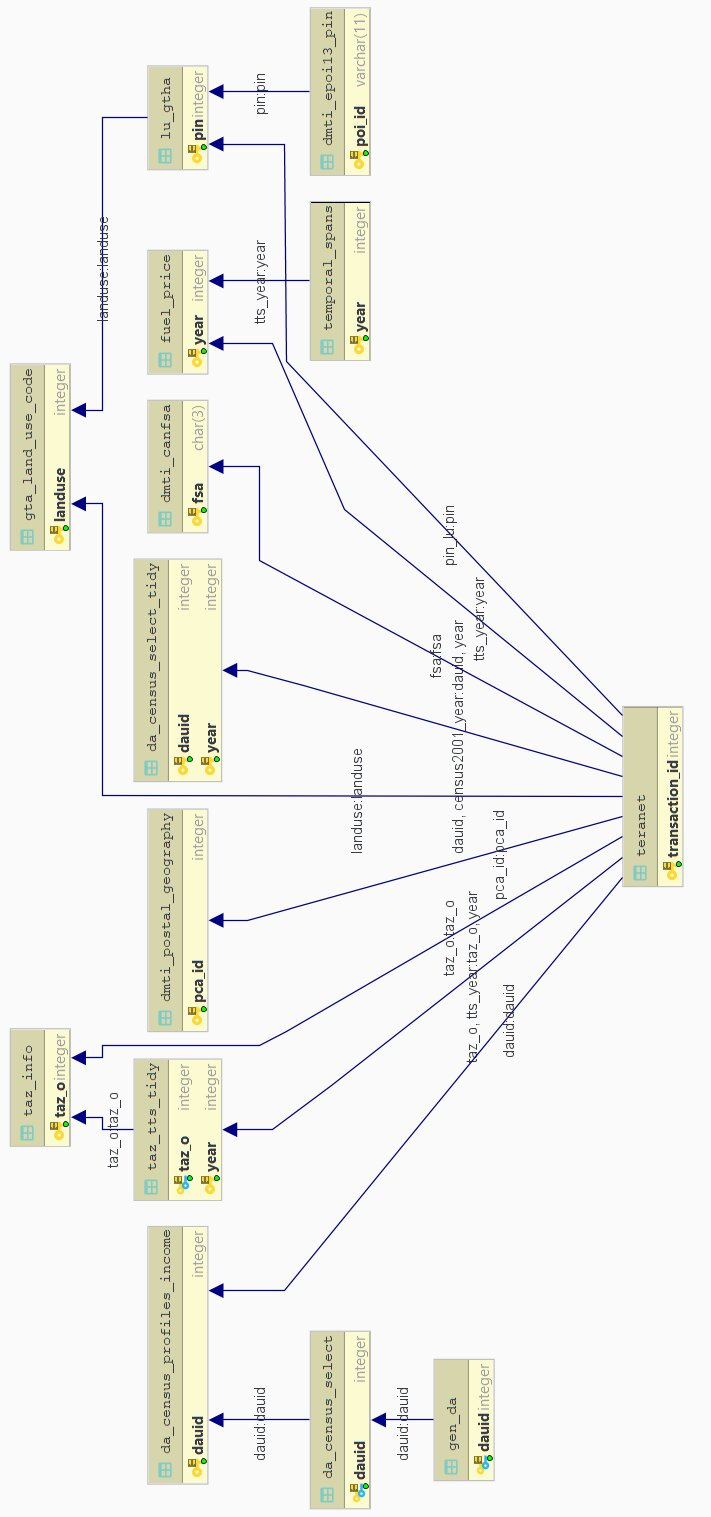
\includegraphics[width=0.65\linewidth,trim=0 0 0 0,clip]{db_schema_vert.jpg}
            \caption{Entity Relationship (ER) diagram for the PostgreSQL database that was implemented as a part of this master's thesis.
            In this database, Teranet dataset augmented with new features and land use produced by the best-performing classification algorithm is combined with related Census and TTS tables.
            Referential integrity constraints were set up to reflect the nature of the spatial and temporal relationships introduced in chapter~\ref{ch:spatial_and_temporal_relationships}}.
            \label{fig:db_schema_vert}
        \end{figure}

    \end{appendices}


%% This adds a line for the Bibliography in the Table of Contents.
\addcontentsline{toc}{chapter}{Bibliography}
%% *** Set the bibliography style. ***
%% (change according to your preference/requirements)
\bibliographystyle{plain}
%% *** Set the bibliography file. ***
%% ("thesis.bib" by default; change as needed)
\bibliography{thesis}

%% *** NOTE ***
%% If you don't use bibliography files, comment out the previous line
%% and use \begin{thebibliography}...\end{thebibliography}.  (In that
%% case, you should probably put the bibliography in a separate file and
%% `\include' or `\input' it here).

\end{document}
